
% Options for packages loaded elsewhere
\PassOptionsToPackage{unicode}{hyperref}
\PassOptionsToPackage{hyphens}{url}
\PassOptionsToPackage{dvipsnames,svgnames,x11names}{xcolor}
\documentclass[10pt]{article}
\usepackage{xcolor}
\usepackage{amsmath,amssymb}
\setcounter{secnumdepth}{3}
\usepackage{iftex}
\ifPDFTeX
  \usepackage[T1]{fontenc}
  \usepackage[utf8]{inputenc}
  \usepackage{textcomp} % provide euro and other symbols
\else % if luatex or xetex
  \usepackage{unicode-math} % this also loads fontspec
  \defaultfontfeatures{Scale=MatchLowercase}
  \defaultfontfeatures[\rmfamily]{Ligatures=TeX,Scale=1}
\fi
\usepackage{lmodern}
\ifPDFTeX\else
  % xetex/luatex font selection
\fi
% Use upquote if available, for straight quotes in verbatim environments
\IfFileExists{upquote.sty}{\usepackage{upquote}}{}
\IfFileExists{microtype.sty}{% use microtype if available
  \usepackage[]{microtype}
  \UseMicrotypeSet[protrusion]{basicmath} % disable protrusion for tt fonts
}{}
\makeatletter
\@ifundefined{KOMAClassName}{% if non-KOMA class
  \IfFileExists{parskip.sty}{%
    \usepackage{parskip}
  }{% else
    \setlength{\parindent}{0pt}
    \setlength{\parskip}{6pt plus 2pt minus 1pt}}
}{% if KOMA class
  \KOMAoptions{parskip=half}}
\makeatother
\usepackage{longtable,booktabs,array}
\usepackage{caption}
\captionsetup[table]{skip=6pt}
\newcounter{none} % for unnumbered tables
\usepackage{calc} % for calculating minipage widths
% Correct order of tables after \paragraph or \subparagraph
\usepackage{etoolbox}
\makeatletter
\patchcmd\longtable{\par}{\if@noskipsec\mbox{}\fi\par}{}{}
\makeatother
% Allow footnotes in longtable head/foot
\IfFileExists{footnotehyper.sty}{\usepackage{footnotehyper}}{\usepackage{footnote}}
\makesavenoteenv{longtable}
\usepackage{graphicx}
\makeatletter
\newsavebox\pandoc@box
\newcommand*\pandocbounded[1]{% scales image to fit in text height/width
  \sbox\pandoc@box{#1}%
  \Gscale@div\@tempa{\textheight}{\dimexpr\ht\pandoc@box+\dp\pandoc@box\relax}%
  \Gscale@div\@tempb{\linewidth}{\wd\pandoc@box}%
  \ifdim\@tempb\p@<\@tempa\p@\let\@tempa\@tempb\fi% select the smaller of both
  \ifdim\@tempa\p@<\p@\scalebox{\@tempa}{\usebox\pandoc@box}%
  \else\usebox{\pandoc@box}%
  \fi%
}
% Set default figure placement to htbp
\def\fps@figure{htbp}
\makeatother
\ifLuaTeX
\usepackage[bidi=basic,shorthands=off]{babel}
\else
\usepackage[bidi=default,shorthands=off]{babel}
\fi
\ifLuaTeX
  \usepackage{selnolig} % disable illegal ligatures
\fi
\setlength{\emergencystretch}{3em} % prevent overfull lines
\providecommand{\tightlist}{%
  \setlength{\itemsep}{0pt}\setlength{\parskip}{0pt}}
\usepackage[]{natbib}
\bibliographystyle{tmlr}
\usepackage{tmlr}
\renewcommand{\arraystretch}{1.35}
\setlength{\extrarowheight}{3pt}
% Table rows in a survey carry paragraphs, not single words, and pandoc's
% longtables set them solid. Both knobs are needed: \arraystretch scales the
% row strut, \extrarowheight lifts the text off the rule above it.
\renewcommand{\arraystretch}{1.35}
\setlength{\extrarowheight}{3pt}
\usepackage{bookmark}
\IfFileExists{xurl.sty}{\usepackage{xurl}}{} % add URL line breaks if available
\urlstyle{same}
% Captions are set a step down from the body, matching the HTML build, where a
% caption is the one block deliberately smaller than the prose around it. The
% caption package is loaded by pandoc's partial above, and only when the paper
% has a table, so this is guarded rather than unconditional: a paper of figures
% and no tables would otherwise fail on an undefined \captionsetup.
\ifdefined\captionsetup\captionsetup{font=small}\fi
% fallback for those not using the hyperref driver hyperxmp:
\makeatletter
\@ifundefined{xmpquote}{\newcommand{\xmpquote}[1]{#1}}{}
\makeatother
\hypersetup{
  pdftitle={From Synchronization Physics to Trained Dynamics: A Survey of Oscillator Networks in Machine Learning},
  pdflang={en-GB},
  pdfkeywords={\xmpquote{coupled oscillators}, \xmpquote{Kuramoto
model}, \xmpquote{reservoir
computing}, \xmpquote{synchronization}, \xmpquote{neural
architectures}, \xmpquote{literature survey}},
  colorlinks=true,
  linkcolor={RoyalBlue},
  filecolor={Maroon},
  citecolor={RoyalBlue},
  urlcolor={RoyalBlue},
  pdfcreator={LaTeX via pandoc}}
% Float placement. LaTeX's defaults reserve most of a page for text, so a
% figure taller than about a third of the block gets deferred, often past the
% section that introduces it: the physics timeline was landing inside the
% neuroscience subsection. These let a float take more of the page it belongs
% on, which keeps figures with the prose that references them.
\renewcommand{\topfraction}{0.92}
\renewcommand{\bottomfraction}{0.85}
\renewcommand{\textfraction}{0.06}
\renewcommand{\floatpagefraction}{0.72}
\setcounter{topnumber}{3}
\setcounter{bottomnumber}{2}
\setcounter{totalnumber}{4}
% Pandoc emits figures with the default [tbp], so a float can only ever move
% forward to the top of a later page. `!htbp` adds "here" and tells LaTeX to
% ignore the size fractions when deciding, which is what actually keeps a tall
% figure in the subsection that introduces it rather than a page or two later.
\makeatletter
\renewcommand{\fps@figure}{!htbp}
\renewcommand{\fps@table}{!htbp}
\makeatother
% A float may drift past the heading that introduces it and read as though it
% belongs to the next one: the physics timeline was landing under "Within
% neuroscience". Flushing pending floats at a heading fixes that. placeins would
% do it, but it is not in a BasicTeX installation, and the mechanism is short:
% if any float is still waiting when a section begins, flush it first.
% \@deferlist holds exactly those floats, so the break only fires when one is
% actually pending.
%
% At \section only, deliberately. Attaching it to every subsection and
% subsubsection clears the page so often that a figure with any text after it
% gets a page to itself: figures 3 and 4 were taking a page each, at 242 and 155
% words of surrounding text. Section-level keeps each figure inside the numbered
% section that cites it, which is what a cross-reference names, and leaves LaTeX
% free to pack the pages in between.
\makeatletter
\newcommand{\tmlr@floatbarrier}{\par\vspace{\z@}%
  \ifx\@deferlist\@empty\else\clearpage\fi}
\let\tmlr@section\section
\renewcommand{\section}{\tmlr@floatbarrier\tmlr@section}
\makeatother

\hypersetup{pdfauthor={}}

\def\month{MM}
\def\year{YYYY}
\def\openreview{\url{https://openreview.net/forum?id=XXXX}}

\title{From Synchronization Physics to Trained Dynamics: A Survey of
Oscillator Networks in Machine Learning}

\author{\name }
\date{}

\begin{document}
\maketitle
\begin{abstract}
Coupled oscillator networks are drawing increased attention as
machine-learning substrates, while at the same time literature from
physics, neuroscience and neuromorphic computing appears to be
converging on the same oscillatory dynamics from different directions.
Physics now describes oscillatory synchronization regimes that exhibit
computation properties rather than mere order. Neuroscience research has
identified the neuron as a complex chemical and physical system with
functional oscillatory properties. The machine learning field has
recently produced oscillator architectures that demonstrate
computational effectiveness on certain tasks such as classification,
image generation and path navigation, even providing evidence to suggest
that oscillatory neural networks (ONNs) can be trained, learn, remember
and reason. Such observations across multiple scientific disciplines are
the motivation for this paper and our overarching hypothesis that an
oscillatory substrate whose native operations are resonance and
entrainment more closely resembles the biological neurons refined
through evolutionary ``training'' to sense and learn from signals in our
physical world, and that a trainable model built from those dynamics
would make questions about learning, forgetting and rhythm disruption
addressable in simulation. We do not aim to test this hypothesis in this
paper, but use it as motivation to provide a critical survey of the
current landscape of ONNs. We organize eighteen published systems, in
fifteen lines, on two questions: whether gradients reach the oscillator
dynamics and whether a conventional encoder or decoder is trained around
it, which separates designed dynamics that are never learned, apparent
learning via untrained dynamics with a trained readout, and trained
dynamics with and without a conventional network wrapped around them.
For each model classification we record the task, the data used, the
controls, and how it compares against conventional artificial neural
network (ANN) baselines at comparable parameter budgets, tasks and
training. The comparative picture is an analysis of parity and niches
rather than a particular architecture's dominance, as the current body
of work on ONNs is, in our opinion, too immature to assert such a
comparison. The evidence surveyed rarely isolates the dynamics: of the
sixty-five applicable control comparisons the five give across the
surveyed systems, sixteen have been run, ten of them by three systems;
the coupling term has been removed as a single variable three times,
once without a reported number, once on a single dataset, and once only
as a retrained model; and no report varies coupling range or boundary
conditions as a single variable. We identify these gaps in greater
detail and close with eight concrete directions for the field that we
believe would help the field establish more cross-referential data,
tasks, training and model architecture parity from which to baseline
future ONN research efforts with more precise controls.
\end{abstract}

\section{Introduction and background}\label{introduction-and-background}

\subsection{What is an oscillator}\label{what-is-an-oscillator}

An \textbf{oscillator} is a system that keeps a rhythm of its own. Left
undisturbed it does not settle at a resting point; it returns to a
closed trajectory, a \emph{limit cycle}, and comes back to that
trajectory after being pushed off it. A clock pendulum, drawing on a
stored energy source to hold its swing against friction, is the familiar
case, and its whole state is one number: how far around the cycle it
currently is, its \textbf{phase}. Models that keep only that number are
\emph{phase-only}, and the Kuramoto and Winfree families this survey
meets most often are of that kind. Models that track an oscillator's
distance from the centre in addition to its phase carry a second
coordinate, the \textbf{amplitude}, so the state lives in a plane rather
than on a circle. The Stuart-Landau equation is the canonical form;
among the systems surveyed here, the second-order recurrences of the
coRNN \citep{rusch2021}, UnICORNN \citep{unicornn} and LinOSS
\citep{rusch2025} lines share that planar state, but as damped or linear
oscillators without the amplitude-restoring term that makes a limit
cycle self-sustaining: started from rest, as all of them are, they
oscillate with whatever amplitude the input gives them rather than
returning to a rhythm of their own. Only coRNN among them is damped in
the model itself; UnICORNN is undamped by construction and LinOSS has no
damping term, a distinction Section 2.3.1 returns to.

\begin{figure}
\centering
\pandocbounded{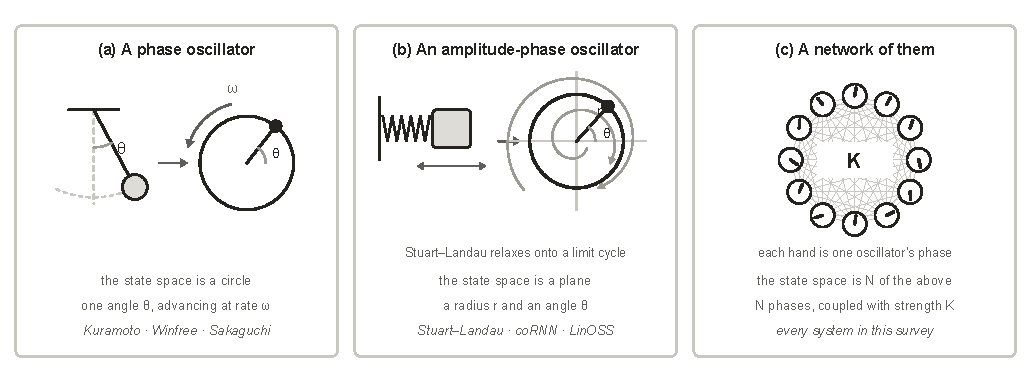
\includegraphics[keepaspectratio,alt={What this survey means by an oscillator, in three widening steps. (a) A phase oscillator keeps a single angle, so its state space is a circle. (b) An amplitude-phase oscillator keeps a radius as well, so its state space is a plane, and trajectories started away from the limit cycle relax onto it. (c) A network keeps N of them and couples each unit to others with strength K. The phases and trajectories drawn are illustrative, not simulated.}]{resources/figures/fig1-oscillator-anatomy.pdf}}
\caption{What this survey means by an oscillator, in three widening
steps. (a) A phase oscillator keeps a single angle, so its state space
is a circle. (b) An amplitude-phase oscillator keeps a radius as well,
so its state space is a plane, and trajectories started away from the
limit cycle relax onto it. (c) A network keeps N of them and couples
each unit to others with strength K. The phases and trajectories drawn
are illustrative, not simulated.}
\end{figure}

\textbf{Coupling} is what makes a population of oscillators one system
rather than many: each unit's rate of change depends on the phases of
the units it is connected to, and the strength of that dependence is the
coupling constant \emph{K}. Where a coupled population settles between
complete lock and complete disorder is measured by the \textbf{order
parameter} \emph{R}, which runs from 0 to 1. Both extremes are useless
for computation. At \emph{R} near 1 every unit does the same thing, so
the population has one degree of freedom left and can carry no signal;
at \emph{R} near 0 nothing is organized for a readout to pick up. The
regime that matters is the partial coherence between them, in which some
units lock while others drift.

\begin{figure}
\centering
\pandocbounded{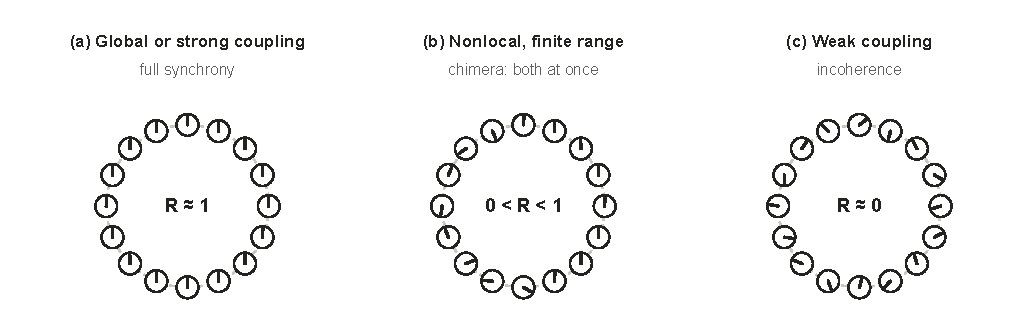
\includegraphics[keepaspectratio,alt={The three coupling regimes reported in the synchronization literature, drawn schematically. Full synchrony leaves no degrees of freedom to carry a signal and incoherence leaves nothing organized; the useful regime is the partial coherence between them, which finite-range nonlocal coupling generically produces. The phases shown are illustrative, not simulated.}]{resources/figures/fig2-coupling-regimes.pdf}}
\caption{The three coupling regimes reported in the synchronization
literature, drawn schematically. Full synchrony leaves no degrees of
freedom to carry a signal and incoherence leaves nothing organized; the
useful regime is the partial coherence between them, which finite-range
nonlocal coupling generically produces. The phases shown are
illustrative, not simulated.}
\end{figure}

That partial regime is also where recurrent computation is reported to
peak. Computation in recurrent networks is maximized near the boundary
between ordered and chaotic dynamics \citep{bertschinger2004},
reservoirs are deliberately parked near that edge, and hierarchical
modular structure makes that edge markedly less sensitive to precise
tuning \citep{kusmierz2025}, a result about autonomous dynamics rather
than about trainability. Every design decision surveyed here, whether
coupling range, damping, spectral placement or sparsity, is a way of
steering the field toward that regime and holding it there, which is
also why the same decisions reappear in Section 3.1 as failure modes.

\subsection{The evolution of oscillator
understanding}\label{the-evolution-of-oscillator-understanding}

Literature from three different fields arrives at similar observations
from different directions. Physics and mathematics come first
chronologically, describing when a coupled population locks and what its
structure does to that. Literature from neuroscience presents findings
that cortex runs on rhythms and uses them to route information.
Applications within machine learning are much more recent, and almost
every system we surveyed aligns with findings from the other two fields.

\subsubsection{Within physics and
mathematics}\label{within-physics-and-mathematics}

The observed coupling of oscillators has been on record since 1665, when
Christiaan Huygens found that two pendulum clocks hung from the same
wooden beam settled into antiphase within about thirty minutes and
resynchronized when disturbed (later published in 1673). Huygens
attributed this to motion too small to see, transmitted through the wood
beam they shared. The prehistory of the self-sustained oscillator runs
from Airy's first mathematical treatment in 1830 through Poincaré's
limit cycle and Blondel's naming of the phenomenon, a lineage traced in
full by \citet{rivera-sierra2026}, whose survey of self-oscillatory
devices for unconventional computing covers similar background as this
paper, but from the materials and neuromorphic hardware angle. Three
centuries after Huygens, his observation was given its mathematical form
by the Kuramoto coupling function \citep{kuramoto1975}, and the same
locking is what a row of metronomes started at different times on a
shared moving platform demonstrates \citep{pantaleone2002}. Huygens'
experiments were later replicated and explained by \citet{bennett2002}.
In biology the same synchronization phenomenon was observed at
population scale and mathematically modelled, from the patterned
flashing of firefly swarms to circadian and cardiac rhythms
\citep{strogatz1993}.

That collective physical dynamics can \emph{be} computation is much more
recent, predating the current oscillatory neural network (ONN) wave by
four decades (\emph{Figure 6}). \citet{hopfield1982} framed memory as
the settling of a dynamic physical system after a stimulus, and argued
that such a system has emergent computational properties.
\citet{mead1990} argued that computing using physics directly is the
efficiency endgame, also inspired by biological adaptations, and the
synchronization canon of \citet{winfree1967}, \citet{kuramoto1975}, the
\citet{strogatz2000} review, and the \citet{pikovsky2001} textbook set
out how coupled oscillator populations self-organize.

Further work on the coupling laws themselves has continued, while the
current ONN landscape in machine learning has not yet caught up. The
single sinusoid was generalized in several directions:
\citet{sakaguchi1986} added a phase lag that breaks the symmetry and
admits partial coherence rather than forcing all-or-nothing locking;
\citet{daido1992} replaced the sinusoid with an arbitrary periodic
function; \citet{schuster1989} put an explicit delay inside the coupling
so that interaction depends on history rather than on the instantaneous
state. Then it was generalized past pairs entirely. \citet{tanaka2011}
coupled three phases at once and found an infinite number of coexisting
synchronized states where pairwise coupling gives one;
\citet{ashwin2016} showed such terms are not an embellishment but what
phase reduction generically produces beyond leading order;
\citet{skardal2019} coupled over simplicial complexes and obtained an
extensive set of stable partially synchronized states; \citet{mulas2020}
did the same over hypergraphs, where a many-body interaction can exist
without its sub-interactions; and \citet{zhang2023} showed those two
representations give qualitatively different synchronization, so
higher-order coupling is at least two distinct generalizations rather
than one. Multistability on such structures is now characterized
directly \citep{bacic2026}. Separately, the oscillator itself was moved
off the circle: \citet{chandra2019} wrote the units as unit vectors in D
dimensions with rotation-matrix natural frequencies, and
\citet{de-aguiar2023} replaced the scalar coupling constant with a
matrix. Appendix C tabulates the full lineage and what each step's
coupling gained over the one before it.

\begin{figure}
\centering
\pandocbounded{\includegraphics[keepaspectratio,alt={Every physics and mathematics source cited in this survey, in date order. The upper track is the account of when a coupled population locks; the lower track is what structure and operating regime do to it. The axis is piecewise, because four entries predate 1930 and most postdate 1990. Almost every machine-learning system in Section 2 takes its coupling law from the upper track, and from the 1967 to 1992 stretch of it in particular. The exceptions are AKOrN {[}@\{akorn\}{]} and, through it, HoloGraph {[}@\{dan2025\}{]}, built on the D-dimensional generalization of @chandra2019 in the lower track. The rest of the lower track is untouched by the surveyed systems, and its earliest two entries are arguments that physics can compute at all rather than coupling laws to build with.}]{resources/figures/fig3-physics-timeline.pdf}}
\caption{Every physics and mathematics source cited in this survey, in
date order. The upper track is the account of when a coupled population
locks; the lower track is what structure and operating regime do to it.
The axis is piecewise, because four entries predate 1930 and most
postdate 1990. Almost every machine-learning system in Section 2 takes
its coupling law from the upper track, and from the 1967 to 1992 stretch
of it in particular. The exceptions are AKOrN \citep{akorn} and, through
it, HoloGraph \citep{dan2025}, built on the D-dimensional generalization
of \citet{chandra2019} in the lower track. The rest of the lower track
is untouched by the surveyed systems, and its earliest two entries are
arguments that physics can compute at all rather than coupling laws to
build with.}
\end{figure}

\subsubsection{Within neuroscience}\label{within-neuroscience}

Neuroscience researchers began observing oscillatory coupling directly
in cortical tissue: neurons in the feline visual cortex oscillate at 40
to 60 Hz and phase-lock across columns when they respond to the same
object, which is why synchrony was proposed as the mechanism binding
distributed features into a single percept \citep{gray1989}.
\citet{fries2015} develops that observation into a ``Communication
through Coherence'' (CTC) hypothesis which essentially states that
inter-neuron communication is selective based on gamma-band coherence
and synchronization.

Reviewing prior studies of mammalian brains, Fries argues that neuronal
groups which need to communicate are tuned to the same gamma band,
roughly 30 to 90 Hz, and synchronize in order to do so: sender and
receiver lock to a common frequency, and inputs arriving at incoherent
phases are effectively ignored. The mechanism he proposes for
establishing those phase relations is entrainment with a conduction
delay, ``both for unidirectional and for bidirectional communication''.
Where it succeeds, ``gamma entrainment allows to transmit a stimulus
representation and to selfishly shut out competing stimuli's
representations'', and it ``establishes a cycle-to-cycle memory of the
active link that maintains until it is terminated at the end of a theta
cycle''. Two features of that account matter here. The gamma rhythm
works because it ``generates fluctuations in network excitation and
inhibition that are sufficiently rapid, such that excitation can
essentially temporally escape its ever chasing inhibition'', so the
useful window is a narrow phase of each cycle rather than a steady
state. And the band itself overlaps the 40 to 60 Hz range at which the
feline visual cortex was found to oscillate and phase-lock, which is
what ties the binding observation and the communication account
together.

Gamma does not act alone. Those bottom-up gamma influences are
themselves modulated by top-down alpha-beta activity at 8 to 20 Hz,
while attention samples the scene at a 7 to 8 Hz theta rhythm that
periodically resets which groups are heard. Communication is therefore
selective not because one rhythm gates it but because several rhythms
interact, and the theta reset means the gating is repeatedly torn down
and rebuilt rather than held.

That last point is what makes the account testable in a network rather
than a brain. If a specific phase and amplitude are required before a
receiving population responds at all, then coupling between groups is
intermittent by construction: groups couple during the excitable window
and decouple after it. Whether the coupling and decoupling of a trained
oscillator network falls into comparable gamma and theta relationships,
and whether it does so on visual tasks in particular, is an open and
directly checkable question, and one Section 3.2 returns to.

Beyond the gamma band, \citet{buzsaki2006} makes the broader claim that
self-emerged oscillatory timing is the brain's fundamental organizer of
neuronal information, and that spontaneous activity is the source of
cognitive capacity rather than noise to be averaged away. The
small-world connectivity of cortex lets these rhythms carry computation
on multiple spatial and temporal scales at once, and the perpetual
interaction between many network oscillators holds the system in a
highly sensitive metastable state, synchronized through weak links at
low energetic cost. At the population level the standard reduction is
the Kuramoto model \citep{breakspear2010}, which, recast as a diffusion
process under the nonlinear Fokker-Planck equation, accounts for two
features of spontaneous large-scale neocortical recordings that a linear
treatment does not: the bistability of the human alpha rhythm, and the
non-Gaussian fluctuations of the beta rhythm. The family of such
reductions, and the mappings between them, has since been set out
systematically \citep{castaldo2026}.

The account is not only about populations. A neuron sitting near its
firing threshold \emph{is} a limit-cycle oscillator, and the
phase-response formalism describing how an input shifts its next spike
is the same one used for coupled oscillators generally, a correspondence
\citet{stiefel2016} set out explicitly. The reductions this rests on
were built for it: \citet{morris1981} keeps two variables of the
\citet{hodgkin1952} conductance dynamics, few enough to analyse and
enough to spike. One consequence matters for everything in Section 2:
cortex is not quiet when undriven. Resting-state functional connectivity
is reproduced by networks of local oscillators running with no stimulus
at all \citep{cabral2011}, which is the biological counterpart of a
field that computes before it is trained.

Sensory transduction offers a sharper precedent, because there the
frequencies are not learned. The cochlea is modelled as a bank of active
oscillators poised near a Hopf bifurcation and tonotopically arranged
\textbf{by design and not by learning} \citep{camalet2000}, an
arrangement that yields the sharp, compressive, actively amplified
tuning measured in real ears \citep{kern2003}. The cochlea therefore
demonstrates something this survey cares about: a bank of oscillators
that performs a hard sensory task well, whose frequencies were fixed by
development rather than fitted to data. Where machine learning would
train those frequencies, biology specifies them.

Speech is where the account is most fully worked out, and it is the
closest thing in neuroscience to a controlled comparison between
oscillator models. Reviewing the field, \citet{dogonasheva2026} set
three families of theta-rhythmic segmentation model against each other
and separate them by where the flexibility to track a variable speech
rate comes from. In the motor-coupled model, auditory and speech-motor
cortices are two phase oscillators coupled in both directions rather
than one driving the other, and the account reproduces the experimental
pattern only once it carries individual differences in the strength of
that auditory-motor connection, which is what makes it a model of
individual variability in speech-rhythm perception rather than of a
population average \citep{assaneo2020}. In the adaptive-frequency model
the oscillator's own natural frequency moves continuously toward the
average period of incoming events, which reproduces human timing
judgements on stimulus sequences whose tone positions are jittered by
about 20\% of the mean period \citep{doelling2023}. In the single-cell
biophysical model, flexibility is intrinsic rather than imposed: the
interaction of an m-current with a super-slow potassium current lets a
Hodgkin--Huxley cell phase-lock across a broad frequency range, and the
resulting segmentation was validated against the TIMIT corpus
\citep{pittman-polletta2021}. What the review says each model cannot
settle is the part relevant here. The two population models are
abstracted away from real neuronal biophysics, so neither can say
whether a cell-level mechanism produces the flexibility they exhibit.
The single-cell model has no network at all and holds its parameters
static, so it cannot say whether a population-level mechanism
contributes. No model in the review spans both levels, so the
flexibility that lets any of them track a variable speech rate cannot
presently be attributed to the cell or to the network. That is
structurally the problem Section 3.1.1 describes on the machine-learning
side, where a system's result cannot be attributed to its oscillator
dynamics because the control that would isolate it has not been run. Two
fields arrived at the same impasse without reference to each other.

Disruption of these rhythms is a recognized signature across
neurological and psychiatric disorders rather than a correlate of one
\citep{uhlhaas2006}, and the relationship has been made interventional:
driving gamma-band activity at 40 Hz reduced amyloid load in a mouse
model \citep{iaccarino2016}.

\textbf{A contested alternative, included because it changes what
``oscillator'' would mean.} The consensus account of the action
potential of a neuron is electrical and conductance-based. A minority
position models it instead as an electromechanical soliton, a density
pulse travelling in the lipid membrane near its melting transition
\citep{heimburg2005}. If something like it held, a neuron would be a
mechanical wave medium rather than a circuit, and the oscillator framing
would be closer to the underlying physics than to a convenient
abstraction. We record it as a live minority hypothesis and take no
position on it: it is contested, it is not what the systems in Section 2
assume, and nothing in this survey depends on it. It is an interesting
supposition nonetheless, and one we would expect continued work on
oscillatory models of cognition to bear on. Were it to hold, the
electrical action potential would be a byproduct of an underlying
electromechanical oscillation rather than the mechanism itself, which
would make the oscillator description of a neuron the literal one rather
than the useful one. We flag that as a direction worth watching and not
as a claim this survey makes or tests.

\begin{figure}
\centering
\pandocbounded{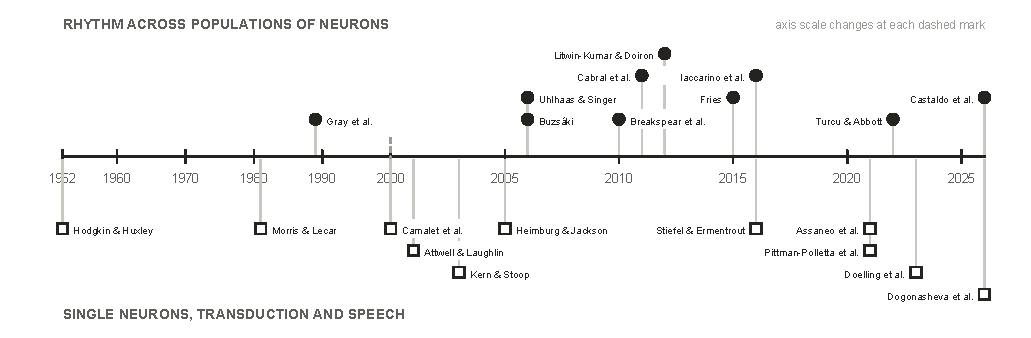
\includegraphics[keepaspectratio,alt={Every neuroscience source cited in this survey, in date order. The upper track is the population account the architectures in Section 2 draw most of their hypotheses from; the lower track is what makes the oscillator description of a neuron literal rather than figurative, together with the transduction and speech work where the frequencies are designed rather than learned.}]{resources/figures/fig4-neuro-timeline.pdf}}
\caption{Every neuroscience source cited in this survey, in date order.
The upper track is the population account the architectures in Section 2
draw most of their hypotheses from; the lower track is what makes the
oscillator description of a neuron literal rather than figurative,
together with the transduction and speech work where the frequencies are
designed rather than learned.}
\end{figure}

Two of the neuroscience findings in this section translate directly into
testable machine-learning claims, and both reappear in Section 3 as
gaps. The binding result \citep{gray1989} predicts that removing the
synchronization term should hurt grouping tasks specifically. The
Hopf-cochlea precedent \citep{camalet2000} predicts that designed
frequency placement should beat learned placement.

\subsubsection{Within machine learning}\label{within-machine-learning}

\textbf{What an oscillator network is.} Section 1.2.1 gives a rule for
how coupled units pull on each other, and Section 1.2.2 gives a reason
to expect that rule to compute something. An oscillator network is what
results when both are pointed at a machine-learning task. An
\textbf{oscillator network}, or oscillatory neural network (ONN), is a
machine-learning system whose state is a population of oscillators and
whose computation is the evolution of that population under a coupling
law. Three choices define one. The \textbf{coupling function} is
borrowed from the physics. It is the rule that turns the phase
difference between two units into a contribution to each one's rate of
change, and choosing Kuramoto rather than Winfree or Sakaguchi fixes
which collective states the population can reach at all; Section 2.3.1
sets the forms actually in use side by side. The \textbf{geometry} is
which units are coupled to which, and it decides both the parameter cost
and the operating regime. The \textbf{input and readout} decide how a
task reaches the field and how an answer is taken out of it. Everything
else is the same machinery any other neural network uses.

Geometry deserves its own picture because it is treated as an
implementation detail in most of the surveyed work and is not one.
All-to-all coupling connects every pair through its own learned weight,
as in Un-0 \citep{un-0}; a ring with a finite coupling range connects
each unit only to units near it; a lattice arranges the units in space
and couples neighbours through a shared kernel, as in Neural Wave
Machines \citep{keller2023} and the convolutional variant of AKOrN
\citep{akorn}; attention connects every pair through weights recomputed
from the current state, as in AKOrN's attentive variant and WONN
\citep{wonn}; a modular fabric is dense inside its blocks and sparse
between them. All-to-all coupling costs O(N\ensuremath{^{2}}) parameters
and is the bulk of the largest system surveyed here. Finite-range
nonlocal coupling is the case in which the physics reports coexisting
locked and drifting domains \citep{kuramoto2002}, which is the regime
Section 1.1 identified as the useful one. And no published work we found
holds a core fixed and varies the geometry, which is why Section 3.1
treats it as an open axis rather than a settled one.

\begin{figure}
\centering
\pandocbounded{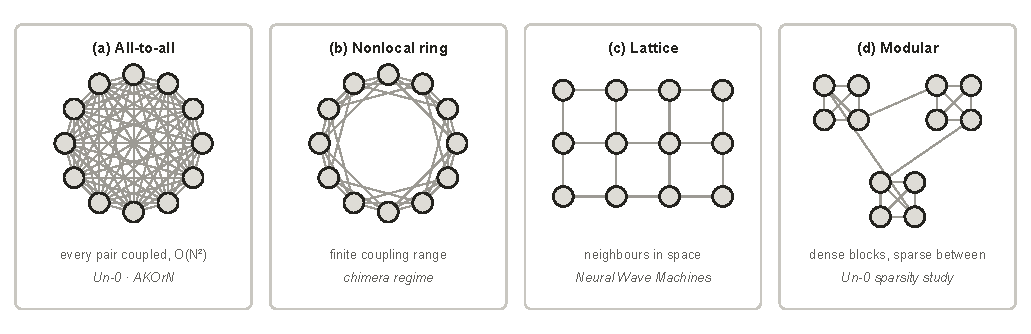
\includegraphics[keepaspectratio,alt={Four coupling geometries over the same twelve oscillators. All-to-all coupling with a free weight per pair is what Un-0 uses, and its O(N) parameter cost is the bulk of Un-0's 322M parameters at 16k oscillators; AKOrN and WONN reach every pair through attention weights instead, and AKOrN's convolutional variant couples a fixed neighbourhood. Finite coupling range is the case the physics canon reports chimera states in. A lattice is the geometry of Neural Wave Machines. The modular fabric is the best performer in the one published sparsity study of a trained oscillator network, which is blog-published and covers one system.}]{resources/figures/fig5-geometries.pdf}}
\caption{Four coupling geometries over the same twelve oscillators.
All-to-all coupling with a free weight per pair is what Un-0 uses, and
its O(N\ensuremath{^{2}}) parameter cost is the bulk of Un-0's 322M
parameters at 16k oscillators; AKOrN and WONN reach every pair through
attention weights instead, and AKOrN's convolutional variant couples a
fixed neighbourhood. Finite coupling range is the case the physics canon
reports chimera states in. A lattice is the geometry of Neural Wave
Machines. The modular fabric is the best performer in the one published
sparsity study of a trained oscillator network, which is blog-published
and covers one system.}
\end{figure}

\textbf{Recent contributions.} The systems fall into three groups by
where the dynamics sits.

\begin{enumerate}
\def\labelenumi{\arabic{enumi}.}
\tightlist
\item
  \textbf{Oscillatory recurrences} replace the recurrence of an RNN with
  a second-order oscillator ODE. The coRNN \citep{rusch2021} is a
  network of coupled, damped, nonlinear oscillators: its hidden units
  interact through full weight matrices inside the nonlinearity, its
  damping bounds the energy of the hidden state, and its gradient bounds
  follow from a structure-preserving discretization under a condition
  that ties the time step to the weight norms, rather than from gating.
  UnICORNN \citep{unicornn} keeps the second-order form but drops both
  the damping and the coupling within a layer: each unit is an
  independent undamped oscillator, y'\,' =
  \ensuremath{-}{[}\ensuremath{\sigma}(w y + Vu + b) +
  \ensuremath{\alpha}y{]} with w a vector applied elementwise, the
  system is Hamiltonian, and a symplectic discretization conserves
  phase-space volume, which is what its gradient bounds rest on; layers
  are stacked densely, each unit carries a trainable time step, and the
  result runs thirty to forty times faster than coRNN. One consequence
  matters for Section 2.3.2: UnICORNN trains nonlinear dynamics with
  full backpropagation through the 17,984-step EigenWorms sequences and
  reaches 90.3\% there, a record set in 2021. Their linear descendants
  trade the nonlinearity for scale: LinOSS \citep{rusch2025} is a bank
  of uncoupled forced harmonic oscillators, y'\,' = \ensuremath{-}Ay +
  Bu + b with A diagonal and no damping term, that is stable for any
  non-negative A, reaches sequences of roughly fifty thousand steps by
  parallel scan, and comes in two discretizations, a conservative one
  and an implicit one whose numerical dissipation the authors read as a
  forgetting mechanism; D-LinOSS \citep{d-linoss} adds an explicit
  learnable damping term and proves that this enlarges the reachable
  dynamics from a measure-zero set of eigenvalues, which the earlier
  discretizations tie to frequency, to the full unit disk. The family
  has universality theorems, and their construction is a fixed bank of
  uncoupled forced harmonic oscillators followed by a nonlinear readout
  \citep{lanthaler2023}; LinOSS proves its own for its continuous-time
  model. Two wording notes are worth recording, because they misled an
  earlier draft of this survey and may mislead a reader. The UnICORNN
  paper twice calls its parameter \ensuremath{\alpha} ``the damping
  parameter'' in its experiments section, while its model section calls
  the same \ensuremath{\alpha} the oscillation frequency and states that
  the system has no damping or friction term; \ensuremath{\alpha}
  multiplies the position, enters the Hamiltonian as the restoring
  potential, and cannot dissipate energy, so we read the model as the
  undamped one its name declares. And the LinOSS paper never uses the
  word damping, while D-LinOSS describes its predecessors as undamped
  harmonic oscillators whose discretization couples frequency and
  damping: the dissipation in question belongs to the implicit
  integrator, not to a term of the model.
\item
  \textbf{Trained synchronization models} put Kuramoto-type dynamics to
  work directly. AKOrN \citep{akorn} uses the D-dimensional
  generalization as a layer inside a conventional network, with the
  coupling defined by a convolution kernel or by attention rather than
  by a free all-to-all matrix, and reports its gains on object
  discovery, adversarial and corruption robustness, calibration and
  Sudoku rather than on clean classification accuracy, where it trails a
  ResNet-18. WONN \citep{wonn} evolves representations on a torus under
  generalized Winfree dynamics, writing the input into the natural
  frequencies rather than adding it as a drive. Its authors describe it
  as the first synchronization architecture to scale competitively to
  ImageNet-1K, and the qualifier matters, since their own table trains
  AKOrN on ImageNet-1K at 67.45\%; it is also the only system in the
  survey evaluated on path finding, and one of two on Sudoku. On
  Maze-hard it reports 76.2\% in a single pass and 80.1\% when the
  lowest-energy of 32 sampled trajectories is selected, at 0.396M
  parameters. The paper frames this as 1\% of the parameters of the
  prior state of the art, but the best result in its own table is
  TRM-Att at 85.3\% with 7M parameters, so the reading we take is a
  model eighteen times smaller that trails the best result by five
  points and beats the 27M-parameter HRM by two to six. Un-0
  \citep{un-0} trains an all-to-all Kuramoto pool end to end for image
  generation and publishes a frozen-dynamics control, a decoder-only
  control and a randomized-structure twin against itself, though only as
  blog posts with released code. KomplexNet \citep{muzellec2025} runs
  Kuramoto dynamics on the phases of a complex-valued CNN's first layer,
  with a coupling kernel trained through a synchrony loss on
  ground-truth object masks, and reports the most complete set of
  controls in the survey: a twin trained without the Kuramoto step, a
  twin whose coupling kernel is held at a fixed Gaussian, and
  parameter-matched real-valued and Transformer baselines. Its headline
  margin of 10 to 15\% over the real-valued model is measured on
  overlapping and noisy digits; in distribution the synchronization step
  is worth two to three points. Kuramoto Attention
  \citep{kuramoto-attention} keeps the query-key selection of an
  attention layer and replaces its value path with a single Kuramoto
  step, and FSN \citep{nunley2026} builds that value pathway from static
  frustration angles, Daido harmonics and an anticipating delay term at
  once, arguing that consensus records where the attended context is
  rather than what followed it, so it suits retrieval but not
  prediction. Kuramoto Orientation Diffusion
  \citep{kuramoto-orientation-diffusion} makes stochastic Kuramoto the
  forward process of a diffusion model, which suits generation on
  periodic domains. HoloGraph \citep{dan2025} swaps the diffusion-style
  message passing of a graph network for synchronization between AKOrN's
  vector-valued oscillators with a feedback term, aimed at the
  over-smoothing repeated diffusion causes; it is the one peer-reviewed
  system in this group whose ablations concern spectral features and
  depth rather than the dynamics. Neural Wave Machines
  \citep{keller2023} replace coRNN's dense coupling matrices with a
  convolution kernel over a lattice, so each oscillator couples only to
  its neighbours, and report travelling waves along with a parameter
  saving that follows from the locality by construction.
\item
  \textbf{Physical substrates} run the dynamics in hardware instead of
  simulating it. A single spin-torque oscillator, time-multiplexed as a
  frozen reservoir, reaches about 99.6\% on spoken digits with one
  device \citep{torrejon2017}. Oscillator Ising machines
  \citep{oscillator-ising-machines} engineer injection locking so the
  physics performs a combinatorial search directly, with no training
  anywhere. Both sit inside the broader physical-reservoir programme
  \citep{tanaka2019}, and the run-the-physics thesis extends past
  oscillators into optical \citep{chen2025} and thermodynamic
  \citep{coles2023} computing. The same ground has been surveyed from
  the materials and device side \citep{rivera-sierra2026}.
\end{enumerate}

\begin{figure}
\centering
\pandocbounded{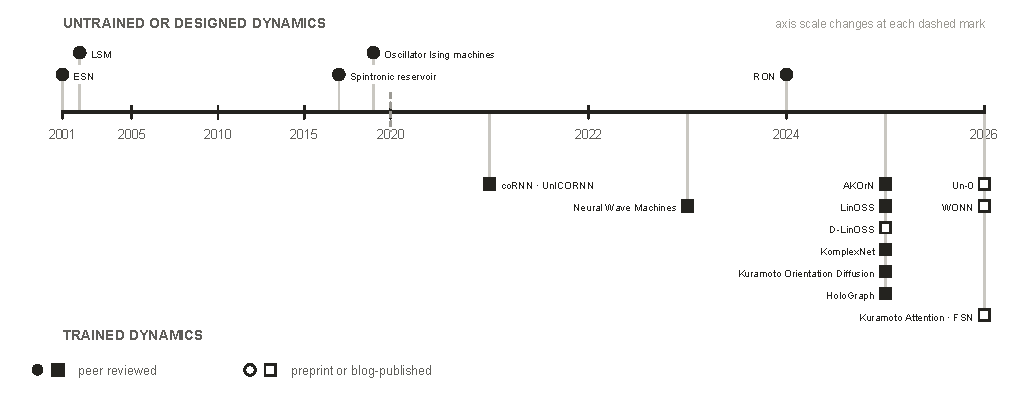
\includegraphics[keepaspectratio,alt={The machine-learning systems this survey covers, by the publication date of the report cited for each. Systems whose dynamics is untrained or designed appear above the axis, systems trained through their dynamics below. A filled marker means the report is peer reviewed. The trained branch is entirely post-2020, and every system whose report is not peer reviewed falls in its last two years.}]{resources/figures/fig6-system-timeline.pdf}}
\caption{The machine-learning systems this survey covers, by the
publication date of the report cited for each. Systems whose dynamics is
untrained or designed appear above the axis, systems trained through
their dynamics below. A filled marker means the report is peer reviewed.
The trained branch is entirely post-2020, and every system whose report
is not peer reviewed falls in its last two years.}
\end{figure}

Set against the physics, the pattern is stark and is one of this
survey's findings. \textbf{Almost every machine-learning system here
uses a coupling law from the 1967 to 1992 window.} Kuramoto and
Kuramoto--Sakaguchi account for nearly all of the trained systems. Past
them the tally is short enough to state exactly. The Stuart-Landau form
appears once \citep{zhang2026}. The D-dimensional generalization appears
once, as the basis of AKOrN. Higher-order coupling appears once, in a
dense associative memory \citep{nagerl2025}. Delay coupling is the
exception, long established in reservoir computing where a single
delayed node stands in for a whole network \citep{appeltant2011}. The
inertial, simplicial, hypergraph and Dirac forms appear not at all.
Swarmalators, in which phase and spatial position couple to each other,
were proposed as a substrate for bio-inspired computing seven years ago
\citep{o-keeffe2019} and we found no machine-learning system built on
them. One of the properties those later models offer is asked for
directly. FSN argues that consensus records where the attended context
is rather than what followed it, and Un-0's sparsity study reports dense
fields collapsing into a globally locked, zero-gradient state, so
partial coherence is a stated requirement of the systems themselves
rather than an inference of ours. Multistability and coupling beyond
pairwise carry no comparable stated demand, and no surveyed system has
tested whether either helps. The gap is untested rather than considered.

\begin{figure}
\centering
\pandocbounded{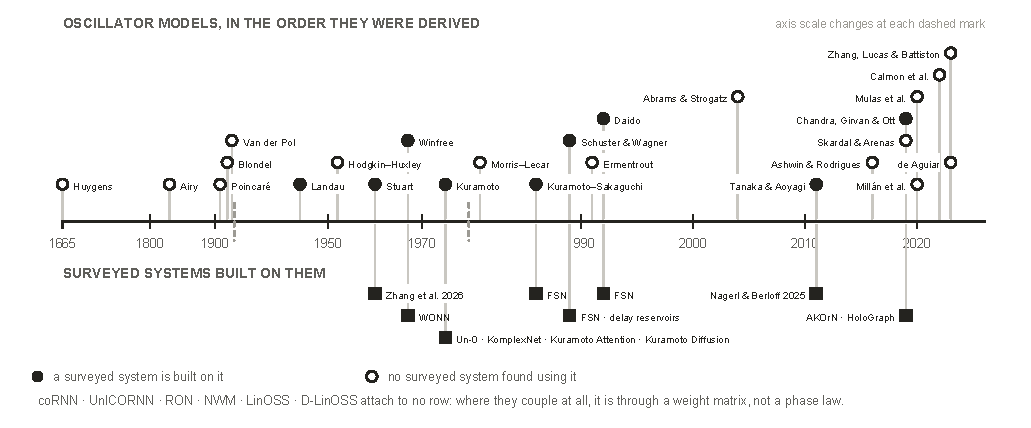
\includegraphics[keepaspectratio,alt={The oscillator models this survey cites, above the surveyed systems built on each one. A filled marker means at least one system in Section 2 uses that coupling form; an open marker means we found none that does. Each system is placed at the year of the model it uses rather than the year it was published, so the lower track measures how far into the lineage the machine-learning literature has reached, not its own chronology.}]{resources/figures/fig7-model-timeline.pdf}}
\caption{The oscillator models this survey cites, above the surveyed
systems built on each one. A filled marker means at least one system in
Section 2 uses that coupling form; an open marker means we found none
that does. Each system is placed at the year of the model it uses rather
than the year it was published, so the lower track measures how far into
the lineage the machine-learning literature has reached, not its own
chronology.}
\end{figure}

\subsection{Other neural network
architectures}\label{other-neural-network-architectures}

Oscillator networks are not the only option, and several of the systems
in Section 2 embed one inside a conventional network rather than
replacing it. Judging what the oscillator dynamics contributes therefore
means knowing what the conventional architectures already do, both as
the baselines an oscillator system is measured against and as the
components it is often combined with. This section sets out the main
families and how each one handles state, which is the property an
oscillator field differs on most.

\textbf{Recurrences carry a state vector forward.} The Elman network
\citep{elman1990} updates a hidden vector once per input and reuses it,
which is the same shape of computation an oscillator field performs,
except that the update is a learned weight matrix rather than a
differential equation. Its failure mode is what every later design
answers: gradients through a long chain of such updates vanish or
explode. The LSTM \citep{hochreiter1997} answers it with gated paths
along which a value passes unchanged, and the gated recurrent unit
\citep{cho2014} reaches the same effect with two gating units where the
LSTM uses four. Oscillator recurrences answer the same question with
different machinery, bounding the gradient through the structure of the
dynamics rather than with gates, a dissipative energy bound and a
structure-preserving discretization in coRNN, conservation of
phase-space volume in UnICORNN, which is why both can prove what an LSTM
can only demonstrate.

\textbf{Convolutions carry no state.} A convolutional network
\citep{lecun1998} applies the same local filter across position and lets
depth build up the receptive field. Weight sharing over a spatial grid
is the assumption an oscillator lattice makes as well; the difference is
that a convolution has no dynamics between applications, so nothing
persists between one input and the next.

\textbf{Attention recomputes over the whole window.} The Transformer
\citep{vaswani2017} drops recurrence entirely and lets every position
attend to every other, which removes the sequential dependency that made
recurrences slow to train. The cost is that it keeps no compressed
state: attention is quadratic in sequence length, and at inference the
keys and values of every previous token must be held in memory, a
footprint that grows linearly with context and dominates serving cost at
scale \citep{kwon2023}. A fixed-size oscillator field is the opposite
trade, which is the substance of the efficiency argument made for it.

\textbf{State-space models put a linear dynamical system back in.} S4
\citep{s4} recovers a constant-size recurrent state while keeping
parallel training, and finds its spectrum's initialization to be
load-bearing rather than incidental \citep{how-train-your-hippo}; Mamba
\citep{mamba} makes the state transition input-dependent and reaches
Transformer-quality language modelling. This is the family the
oscillatory recurrences are closest to: LinOSS \emph{is} a state-space
model whose transition is a bank of harmonic oscillators, which is why
it is also the oscillator system with the longest gradient horizon in
the survey, roughly fifty thousand steps; UnICORNN's 17,984 is the
longest for a nonlinear one. Hybrids interleave the two, keeping a few
attention layers for recall over a mostly recurrent stack
\citep{lieber2024}.

\textbf{Spiking networks are the nearest neighbour.} A spiking unit is
an oscillator of a restricted kind: it integrates input, crosses a
threshold, emits a discrete event, and resets. That discreteness is what
makes it efficient on neuromorphic hardware and what makes it hard to
train, since the threshold is non-differentiable, so gradient methods
need a surrogate and the choice of surrogate is itself a modelling
decision \citep{neftci2019}. Oscillator models keep the state
continuous, so coupling is differentiable and no surrogate is needed,
and they carry structure a threshold unit discards: a natural frequency,
a phase relationship to every other unit, and a graded rather than
binary response to input. Recent work narrows the gap from the other
side, training networks of Morris--Lecar neurons directly with
backpropagation \citep[preprint]{akbari2025}. \textbf{Whether continuous
state makes oscillator networks easier to train is open, and this
survey's own evidence cautions against assuming it.} No published work
compares a spiking network and an oscillator network on one task under
matched conditions, and every nonlinear oscillator system in the record
that lacks a proven gradient bound works at a short gradient horizon
(Section 2.3).

\begin{figure}
\centering
\pandocbounded{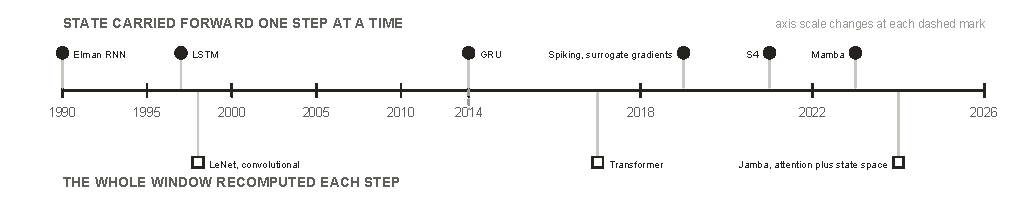
\includegraphics[keepaspectratio,alt={Conventional neural network architectures, by how each one holds the past. Above the axis, a state is carried forward one step at a time; below it, the whole window is recomputed at every step. An oscillator field belongs to the upper track, but its state evolves under a fixed differential equation rather than under a transition learned from scratch, which is the substance of both the efficiency argument made for it and the training difficulty reported against it.}]{resources/figures/fig8-ann-timeline.pdf}}
\caption{Conventional neural network architectures, by how each one
holds the past. Above the axis, a state is carried forward one step at a
time; below it, the whole window is recomputed at every step. An
oscillator field belongs to the upper track, but its state evolves under
a fixed differential equation rather than under a transition learned
from scratch, which is the substance of both the efficiency argument
made for it and the training difficulty reported against it.}
\end{figure}

\subsection{Motivation for this survey: independent convergence across
fields}\label{motivation-for-this-survey-independent-convergence-across-fields}

The case for reviewing oscillator networks is not that any single result
is decisive. It is that literatures with different methods and
incentives have moved toward the same description of computation,
coupling and coherence, and did so largely without citing each other.

\textbf{From physics}, the synchronization canon now describes regimes
that look like computation rather than mere order: partial coherence,
chimera states with locked and drifting populations coexisting in one
field \citep{abrams2004}, multistability on higher-order interaction
structures, and a computational optimum near the boundary between order
and chaos. \textbf{From neuroscience}, the oscillator description of a
neuron has hardened from analogy into working model, rhythm has been
given specific computational jobs, and disruption of those rhythms is
now interventional rather than merely descriptive. \textbf{In machine
learning}, oscillator dynamics has begun to appear in architectures that
run on mainstream tasks at non-trivial scale: 76.78\% top-1 on
ImageNet-1K at 12.3M parameters (WONN, preprint), class-conditional
generation on ImageNet-64 at FID 6.74 (Un-0, blog-published), regression
over fifty-thousand-step windows (LinOSS), object discovery and Sudoku
(AKOrN), and character- and byte-level language modelling (Kuramoto
Attention, preprint). What these results establish is that the dynamics
can be trained at these scales at all; the long-sequence result has a
2021 precedent in UnICORNN's 17,984-step classification, and the rest
were not on the record five years ago. What they do not establish is how
the systems stand against tuned conventional baselines, which Section
2.3.4 takes up.

The machine-learning literature has so far built on the simpler end of
that physics, and it is already getting results there. The coupling laws
in use generally end around the 1992-era physics models (Figure 7), and
the geometries in the surveyed machine-learning models are all-to-all,
convolutional or attention-defined, with Un-0's sparsity study the only
one to vary connectivity on purpose, while the more recent physics
models demonstrate behaviour ONN researchers have reason to want.
Partial coherence is the clearest case: two of the surveyed systems name
full synchronization as the failure mode they are trying to avoid.
Multistability and coupling beyond pairwise are untried here rather than
unwanted. That gap reads as headroom rather than deficiency: more
expressive coupling laws are sitting unused, and the results already
obtained with the simple ones are the reason to think the richer ones
are worth trying.

Three motivations sit behind the interest, and they are worth separating
from evidence:

\begin{enumerate}
\def\labelenumi{\arabic{enumi}.}
\tightlist
\item
  \textbf{Energy and compute}. The brain's signalling budget is small
  enough to be a standing reproach to conventional accelerators
  \citep{attwell2001}, and running physics directly has been the
  efficiency argument since \citet{mead1990}; the concrete modern
  version is that a fixed-size dynamical state avoids the growing
  key-value cache that dominates Transformer serving. \textbf{No trained
  oscillator network has published a measured energy win} (Section
  2.3.4), so this is a reason to look, not a result.
\item
  \textbf{Alignment with the signals}. The signals biological sensing
  evolved to handle are physical waves, and the transducers that receive
  them are frequency-selective by construction, the cochlea being the
  clearest case. A substrate whose native operations are resonance,
  entrainment and phase relationship is therefore not an arbitrary
  inductive bias for these signals; it is the same class of object as
  the thing being sensed.
\item
  \textbf{Explanatory}: a trainable model built from the same dynamics
  as the biological account would make questions about learning,
  forgetting and rhythm disruption addressable in simulation. All three
  are hypotheses about what the field could deliver. This survey is
  about what it has delivered.
\end{enumerate}

\subsection{Evidence standard and
limitations}\label{evidence-standard-and-limitations}

\textbf{Evidence standard.} This survey reports no new experiments and
cites no unpublished results. Every claim is attributed to a published
source. A substantial part of the trained-Kuramoto evidence exists only
as technical blog posts, preprints, or community repositories. That
material is included, because excluding it would misrepresent the state
of the field, and it is marked as non-peer-reviewed everywhere it
carries weight. Where a claim rests on such a source, the text says so
at the point of use rather than in a footnote.

Five limitations bound every claim that follows.

\begin{enumerate}
\def\labelenumi{\arabic{enumi}.}
\tightlist
\item
  \textbf{Publication-status heterogeneity.} The strongest evidence that
  trained pure-Kuramoto dynamics works at scale, and all of the
  oscillator-sparsity evidence, is blog-published. Several load-bearing
  systems are preprints: WONN \citep{wonn}, Kuramoto Attention
  \citep{kuramoto-attention}, FSN \citep{nunley2026}, and the
  equilibrium-propagation study \citep{ahmadi2026}. KomplexNet
  \citep{muzellec2025} is the one system in this group to have completed
  peer review since we began this survey, which is itself a reminder of
  how quickly the status of any row here can change. Independent
  replications are essentially absent field-wide.
\item
  \textbf{Protocol heterogeneity.} Numbers quoted from different papers
  cannot be fairly compared across models and protocols. They are
  therefore set beside each other observationally in this survey and
  never ranked.
\item
  \textbf{Coverage bounds.} We survey the machine-learning-facing
  evidence. The synchronization physics, neuroscience and hardware
  literatures are cited as anchors for background and motivation, and
  were not reviewed exhaustively.
\item
  \textbf{A fast-moving field.} Every ``lacks evidence'' claim carries
  an implicit ``that we found''. Several systems surveyed here are
  months old, and there may be work under review addressing the gaps we
  identify.
\item
  \textbf{Interest disclosure.} The authors conduct their own
  experimental work on oscillator substrates. The gaps identified
  reflect those interests. No unpublished work of ours is used or cited.
\end{enumerate}

\section{Oscillator neural networks}\label{oscillator-neural-networks}

\subsection{Scope and terms}\label{scope-and-terms}

A ``coupled oscillator network'' here means a machine-learning system
whose state evolves under oscillator dynamics: phase-only models of the
Kuramoto and Winfree family, second-order oscillator ODEs, linear
oscillatory state-space models, amplitude-phase models, and physical
oscillator hardware. Eighteen load-bearing systems meet that definition
and are tabulated in Appendix D as fifteen rows, since three pairs share
an architecture and a control record: the echo-state network and the
liquid state machine, LinOSS \citep{rusch2025} and D-LinOSS
\citep{d-linoss}, and Kuramoto Attention \citep{kuramoto-attention} and
FSN \citep{nunley2026}. The same words are used differently in physics,
neuroscience and machine learning, and several of the comparisons below
depend on which sense is meant; Appendix B is a glossary of the terms as
this survey uses them.

One adjacent literature is deliberately outside that definition. A
substantial body of work uses neural networks to \emph{model} oscillator
dynamics rather than to compute with them, learning the evolution of a
coupled system from data, most recently through Koopman operator methods
\citep{sasikumar2026}. That is the inverse of the question here. This
survey asks what oscillator dynamics does for a machine-learning system,
not what a machine-learning system can say about oscillator dynamics.

\subsection{Taxonomy}\label{taxonomy}

\subsubsection{Overview}\label{overview}

Two independent questions separate the surveyed systems, and crossing
them gives four quadrants rather than a tree. The first is
\textbf{whether gradients reach the dynamics}: is the oscillator field
fitted to the task, or fixed by design or at random before training
begins? The second is \textbf{whether anything else is trained}: does a
conventional encoder, decoder or readout sit around the field and do
part of the work? The first question is where the field's claims differ
most. The second is where its attribution problems live, because a
trained scaffold can carry a result that is then reported as the
dynamics'.

\begin{figure}
\centering
\pandocbounded{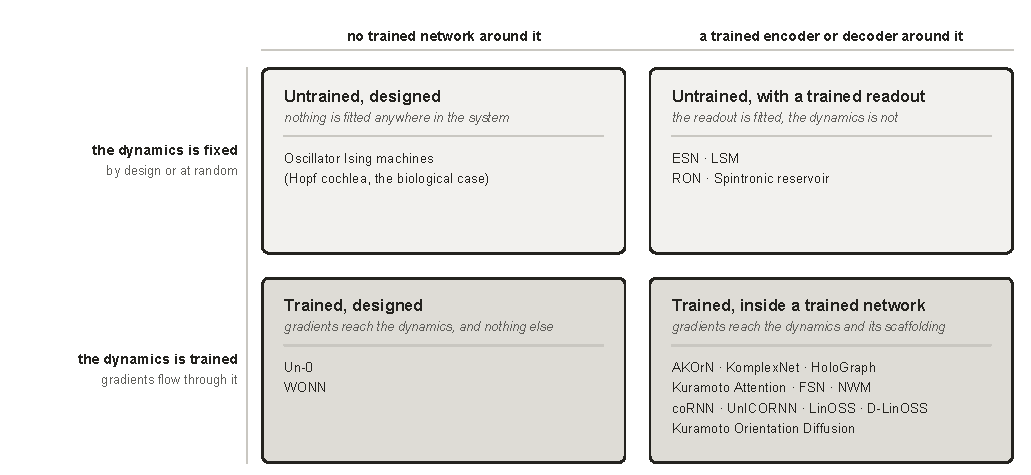
\includegraphics[keepaspectratio,alt={The taxonomy used in this survey. Systems split on two independent questions: whether gradients reach the dynamics, and whether a trained conventional network wraps it. Coupling law, geometry and substrate cut across all four quadrants and are carried as columns in Section 2.3 rather than as further branches, because nesting them produces a tree no system occupies uniquely.}]{resources/figures/fig9-taxonomy.pdf}}
\caption{The taxonomy used in this survey. Systems split on two
independent questions: whether gradients reach the dynamics, and whether
a trained conventional network wraps it. Coupling law, geometry and
substrate cut across all four quadrants and are carried as columns in
Section 2.3 rather than as further branches, because nesting them
produces a tree no system occupies uniquely.}
\end{figure}

\subsubsection{Untrained designed
dynamics}\label{untrained-designed-dynamics}

Nothing is fitted anywhere. Every parameter is chosen, and the physics
performs the computation directly. Oscillator Ising machines
\citep{oscillator-ising-machines} are the clear case: injection locking
is engineered so that the equilibrium the hardware falls into is the
answer to a combinatorial problem, and there is no training step of any
kind. This is the strongest form of the run-the-physics argument: if a
system's parameters can be chosen so that its natural dynamics settles
on the answer, the computation costs whatever the physics costs and no
more. It is also why designing a substrate around a specific task,
rather than training a general one to perform it, should be further
studied by the field.

The biological precedent sits in the same quadrant and is worth keeping
in view because it is the one place where designed beats learned on the
record. The cochlea is a tonotopically arranged bank of active
oscillators whose frequencies are set by construction, not fitted, and
it delivers sharp, compressive, actively amplified tuning that no
learned filterbank has bettered.

\subsubsection{Trained designed
dynamics}\label{trained-designed-dynamics}

Gradients reach the dynamics, and the dynamics is essentially the whole
model rather than a component of one; a thin conventional encoder or
decoder may remain, and in Un-0 it is under 13\% of the parameters. Un-0
\citep{un-0} is a pure Kuramoto pool with learned all-to-all coupling
and learned natural frequencies, read out by a convolutional decoder and
trained end to end for image generation; WONN \citep{wonn} uses
generalized Winfree coupling, writes the input into the natural
frequencies through a learned embedding rather than adding it as a
drive, and updates those frequencies once per layer. Both are the
field's scale demonstrations, and both are also where the attribution
question is cleanest, because there is comparatively little conventional
machinery to which a result could be misattributed, which is also what
makes a decoder-only control meaningful for Un-0. Un-0 publishes the
controls this quadrant makes possible: a frozen-reservoir control,
against which its trained dynamics wins clearly, with single-step
learned dynamics performing near the untrained level on CIFAR-10, and a
decoder-only control that does worse than either (blog-published). WONN
publishes neither.

\subsubsection{Untrained dynamics with a trained encoder or
decoder}\label{untrained-dynamics-with-a-trained-encoder-or-decoder}

The dynamics is fixed, randomly or by design, and a readout is fitted to
it. This is the oldest branch and the best evidenced, because a field
was built on it: echo-state networks and liquid state machines fix
random recurrent dynamics and train only a linear readout
\citep{jaeger2001, maass2002}, a construction whose scope and limits
were consolidated a decade later \citep{lukosevicius2009}.

The oscillator-specific evidence here is the strongest in the survey. A
single physical spin-torque oscillator, time-multiplexed as a frozen
reservoir, reaches roughly 99.6\% spoken-digit recognition with one
device rather than a network of them \citep{torrejon2017}. Untrained
networks of randomly coupled damped oscillators, RON \citep{ceni2024},
are reported to beat a leaky echo-state network on every benchmark they
run, and to beat fully trained recurrent models, including a trained
version of themselves, on chaotic forecasting and on small-parameter
classification, while losing to the trained models on the long-memory
classification tasks; the trainable parameters are matched, which the
paper enforces, and the random reservoir then carries about fifty times
more units than the trained networks. That is a trained-versus-untrained
comparison in the untrained direction, and the paper's trained twin is
the frozen-twin control of Section 2.3.3 run in reverse. And designed
dynamics can replace random dynamics at no cost: deterministic
minimum-complexity reservoirs match classical random echo-state networks
\citep{rodan2011}.

The distinguishing feature within this quadrant is \textbf{where the
fixed dynamics comes from}, and it matters because Section 3.1 shows
designed structure repeatedly failing to beat randomized twins
elsewhere. Random initialization is the reservoir default, deterministic
construction is a documented alternative at equal accuracy, and the
tonotopic cochlea is the limiting case in which every parameter is
chosen. This is the one branch where that comparison has been run and
design holds up.

\subsubsection{Trained dynamics with a trained encoder or
decoder}\label{trained-dynamics-with-a-trained-encoder-or-decoder}

Gradients flow through the oscillator dynamics \emph{and} through
conventional layers around it. This quadrant drives the current wave and
carries the heaviest attribution burden, since a conventional scaffold
surrounds the part under test.

Within it, the useful sub-division is \textbf{architectural role},
because it predicts both the training horizon and the controls the
system needs. As a \textbf{recurrent core}, the dynamics replaces the
recurrence of an RNN: coRNN \citep{rusch2021} and UnICORNN
\citep{unicornn}, LinOSS \citep{rusch2025} and D-LinOSS
\citep{d-linoss}, and Neural Wave Machines \citep{keller2023}. This is
where the theory is strongest and the horizons longest. As a
\textbf{layer inside a conventional network}, Kuramoto dynamics sits as
one block among ordinary ones: AKOrN \citep{akorn}'s D-dimensional
layers, KomplexNet \citep{muzellec2025}'s phase dynamics inside a
complex-valued CNN, the synchronization message passing of HoloGraph
\citep{dan2025} inside a graph network. As an \textbf{attention
mechanism}, a Kuramoto or Kuramoto--Sakaguchi step stands in for an
attention layer, typically one dynamics step per layer: Kuramoto
Attention \citep{kuramoto-attention} and FSN \citep{nunley2026}. As a
\textbf{generative process}, stochastic Kuramoto becomes the forward
process of a diffusion model trained through per-step score objectives
rather than through a long chain: Kuramoto Orientation Diffusion
\citep{kuramoto-orientation-diffusion}.

The theory underwriting this quadrant is real and worth stating, because
it establishes that the function class is there to be learned even where
the evidence that it \emph{is} learned is thin. The family is universal,
with quantitative approximation and generalization bounds
\citep{huang, huang2025} and an infinite-horizon extension
\citep{sagodi}; input-to-state stability has been established for
coupled oscillator networks \citep{stolzle2024}; and contraction
conditions are known for composing stable recurrent modules
\citep{kozachkov2022}. One result cuts the other way, and it is the
sharpest thing theory says here: within-layer coupling may not be
required for the family's universality, because a diagonal, uncoupled
bank could suffice \citep{lanthaler2023}. That is proved for a fixed
bank of forced harmonic oscillators with a nonlinear readout, in
continuous time, rather than for the Kuramoto-family models most of the
surveyed systems use, and a discretization inherits it only for small
time steps, so it bounds what synchronization can be claimed to add
rather than settling it. If it carries, whatever synchronization
contributes is inductive bias, and only a controlled ablation can
measure it.

\subsection{Comparison of the current
landscape}\label{comparison-of-the-current-landscape}

\subsubsection{What the systems are built
from}\label{what-the-systems-are-built-from}

Appendix D records what each system \emph{is}: its oscillator family,
the part of a model the dynamics constitutes, what gradients reach, and
whether the work is peer reviewed. Appendix E records what each system
\emph{reports}: task, data, headline result, parameter count and
training horizon. Both are inventory. The three things worth reading
across them are the coupling law, the geometry, and where the input
enters, because those are the choices the physics says are consequential
and the papers make in passing.

\begin{figure}
\centering
\pandocbounded{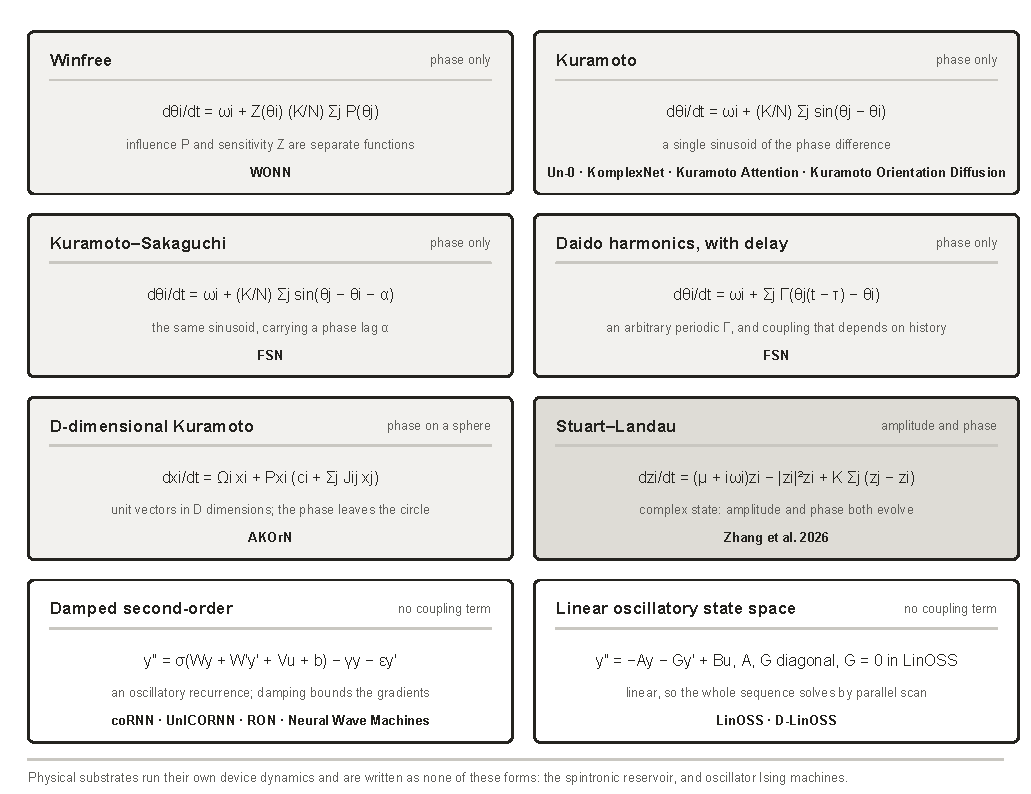
\includegraphics[keepaspectratio,alt={The oscillator dynamics each surveyed system is built on, grouped by how the dynamics is written rather than by when it was published. The first seven forms carry a coupling term between units, whether as a phase difference, a projected vector sum, or, in the coupled second-order recurrences, full or convolutional weight matrices inside the nonlinearity. The last two do not: UnICORNN's units are independent within a layer and LinOSS's state matrices are diagonal, which is why Section 2.3.3 records a coupling ablation for those rows as not applicable rather than as missing. Appendix C places all of them in the wider lineage.}]{resources/figures/fig10-model-lineage.pdf}}
\caption{The oscillator dynamics each surveyed system is built on,
grouped by how the dynamics is written rather than by when it was
published. The first seven forms carry a coupling term between units,
whether as a phase difference, a projected vector sum, or, in the
coupled second-order recurrences, full or convolutional weight matrices
inside the nonlinearity. The last two do not: UnICORNN's units are
independent within a layer and LinOSS's state matrices are diagonal,
which is why Section 2.3.3 records a coupling ablation for those rows as
not applicable rather than as missing. Appendix C places all of them in
the wider lineage.}
\end{figure}

\textbf{Where the input enters} looks like an implementation detail and
is not one. Classical theory is unambiguous that input can only pull the
phases into step if it acts on the phase, so an additive drive and a
value written into the natural frequency do different things
(\citet{adler1946}; the phase-response formalism in
\citet{pikovsky2001}), and drive competes with mutual order in forced
populations \citep{childs2008}. Hardware treats injection locking as the
computation itself. The surveyed systems scatter across the four
available forms silently: additive drive (LinOSS; coRNN, inside its
nonlinearity), phase-coupled conditioning (AKOrN's projected
conditioning, Un-0's conditioning oscillators sin-coupled into the
field), input written into natural frequencies (WONN), and input-gated
coupling strength (KomplexNet). No paper in this set contrasts two
injection forms under controls or discusses the choice as a choice.

\begin{figure}
\centering
\pandocbounded{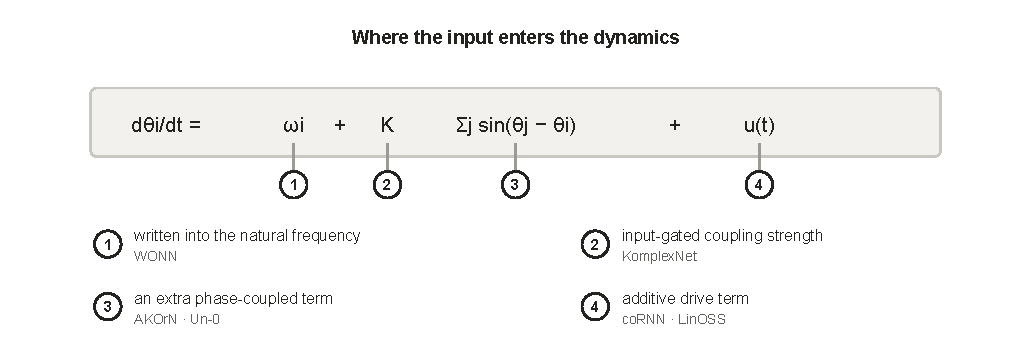
\includegraphics[keepaspectratio,alt={The four ways input enters the dynamics across the surveyed systems, each marked against the term it modifies. Classical theory makes this consequential rather than incidental: entrainment requires a phase-dependent term, so writing input into the natural frequency (1) and adding it as a drive (4) are not interchangeable. No paper in this survey contrasts two injection forms under controls.}]{resources/figures/fig11-input-injection.pdf}}
\caption{The four ways input enters the dynamics across the surveyed
systems, each marked against the term it modifies. Classical theory
makes this consequential rather than incidental: entrainment requires a
phase-dependent term, so writing input into the natural frequency (1)
and adding it as a drive (4) are not interchangeable. No paper in this
survey contrasts two injection forms under controls.}
\end{figure}

\textbf{Geometry and capacity} are separable design choices in
principle, and whether they can be set separately in practice is not
something the record answers: one surveyed system has varied them
together; none has varied either alone. Un-0's sparsity study
\citep{sparsity-study} reports that static masks fixed before training
remove 50 to 98.4\% of couplings and maintain or \emph{improve}
generation; that at the smallest ImageNet-64 size the best result is a
modular variant at reduced parameter count; that optimal sparsity scales
with system size; and that above a critical sparsity performance
degrades, the extreme failure being input-output disconnection. Its own
summary is that connectivity acts as a control knob, not a monotonic
regularizer. Two attributions carry independent interest: improvements
track generative \emph{recall}, meaning diversity, rather than
precision, under the established decomposition
\citep{sajjadi2018, kynkaanniemi2019}, and sparse systems tolerate
higher learning rates, with dense failures blamed on collapse into
global lock. All of this is blog-published, one system, one modality.
The physics is consistent with it: chimera coexistence is generic for
nonlocal finite-range coupling, modular fabrics natively produce
chimera-like states and metastable timescale hierarchies
\citep{hizanidis2016, litwin-kumar2012}, sparse recurrent fabrics
classify at high capacity through resonant amplification
\citep{turcu2022}, and in conventional networks near-independent
recurrent modules generalize better out of distribution
\citep{goyal2021} while spatial wiring costs make modularity emerge
\citep{achterberg2023}.

\textbf{Damping and frequency placement} are the two physics parameters
the surveyed papers do report, and each turns out to be doing two jobs
at once. The spectral radius of an echo-state network is simultaneously
its stability condition and its memory-nonlinearity operating point;
coRNN's damping bounds the energy of its hidden state, which its
gradient analysis then rests on, while its authors offer only heuristics
and a robustness sweep on what damping does for expressivity; D-LinOSS
learns its damping to widen the reachable spectrum, and keeps its
eigenvalues inside the unit disk by constraining the frequency given the
damping and time step rather than by the damping itself; and a
speech-oscillator study built on coRNN sweeps its frequency and damping
ranges together and finds the low-frequency band decisive
\citep{chandravadia2026}. Frequency placement shows the
design-beats-training pattern repeatedly: state-space models find their
spectrum's initialization load-bearing, D-LinOSS initializes in spectrum
space by design, envelope-band initialization decides success on
raw-waveform speech, and the cochlea literature designs the bank
outright.

\subsubsection{What the systems are evaluated
on}\label{what-the-systems-are-evaluated-on}

A survey of this shape would normally open its comparison with a shared
benchmark. The field has not established one yet, and that absence is
itself one of the gaps this survey identifies. Some convergence has
started: Sudoku is now reported by two independent groups, AKOrN and
WONN, and CIFAR and ImageNet recur across several systems, though at
different tasks. The spread is still the point, though. Read down the
task column of Appendix E: class-conditional image generation scored by
FID, ImageNet-1K top-1 classification, maze path finding and Sudoku,
object discovery, multi-object binding robustness at small scale,
character-level language modelling, generation on periodic domains,
extreme-length sequence classification, general time-series benchmarks,
spoken-digit recognition, and combinatorial optimization. Almost no two
rows share a task, and where two rows do, they rarely share a protocol.

Shared cross-disciplinary benchmarks largely do not exist here for three
reasons. The field is genuinely multidisciplinary: results arrive from
nonlinear dynamics, neuromorphic hardware, computational neuroscience
and mainstream deep learning, and each of those communities brought its
own evaluation habits with it. A physics group reporting a locking
diagram and a deep-learning group reporting top-1 accuracy are not being
careless with each other's conventions; they are answering different
questions. The field is also young. Most of the trained-dynamics systems
here postdate 2023, and a subfield converges on shared benchmarks once
its methods stabilize, not before. And the substrates are not
commensurable: a time-multiplexed physical oscillator and a
322M-parameter simulated Kuramoto pool cannot be run on one task suite
even in principle.

As a result, cross-system accuracy comparisons are unsafe, because the
tasks differ and so does the effort spent tuning each baseline. A
general claim of the form ``oscillator networks are better at X'' cannot
be supported by this record, because no two systems have been run on X
under one protocol. Narrower claims can be made, and two papers make
them: Kuramoto Attention reports beating a parameter-matched Transformer
at the 5M scale on byte-level code, and RON reports beating echo-state
and fully trained recurrent baselines on chaotic forecasting. Each of
those stands for its own task at its own scale against its own baseline.
What does not follow from either is that the result carries to another
task, another parameter budget, or another oscillator system. And an
absent result is not a demonstrated limitation: generative speech,
streaming inference and measured energy on hardware contain no
oscillator system at all, so nothing has been shown to fail there.

\begin{figure}
\centering
\pandocbounded{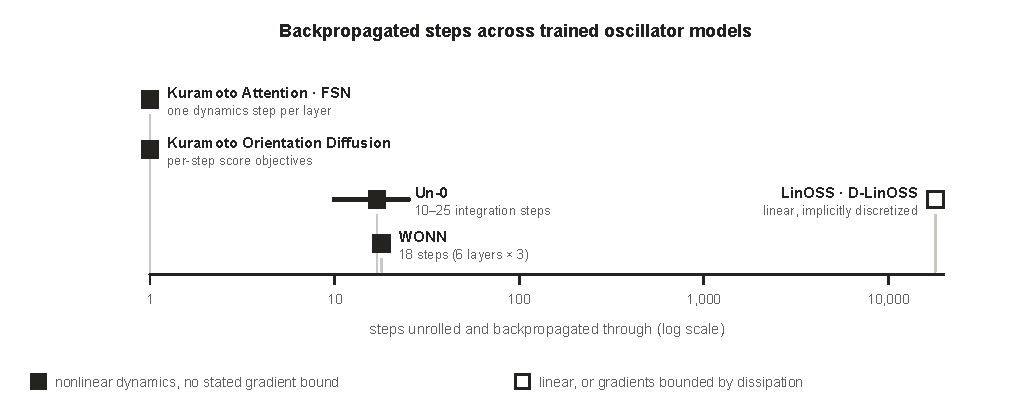
\includegraphics[keepaspectratio,alt={Steps unrolled and backpropagated through, by system. Filled markers are nonlinear dynamics with no stated gradient bound; half-filled markers are nonlinear dynamics whose gradients are controlled by the structure of the dynamics, a dissipative energy bound with a time-step condition in coRNN and Neural Wave Machines, and Hamiltonian conservation in UnICORNN; the open marker is linear dynamics. Every nonlinear system without a stated bound trains at twenty-five steps or fewer; the two nonlinear systems that reach thousands of steps carry a proof, and the only system beyond twenty thousand is linear.}]{resources/figures/fig12-training-horizon.pdf}}
\caption{Steps unrolled and backpropagated through, by system. Filled
markers are nonlinear dynamics with no stated gradient bound;
half-filled markers are nonlinear dynamics whose gradients are
controlled by the structure of the dynamics, a dissipative energy bound
with a time-step condition in coRNN and Neural Wave Machines, and
Hamiltonian conservation in UnICORNN; the open marker is linear
dynamics. Every nonlinear system without a stated bound trains at
twenty-five steps or fewer; the two nonlinear systems that reach
thousands of steps carry a proof, and the only system beyond twenty
thousand is linear.}
\end{figure}

\textbf{What is comparable.} Two kinds of comparison survive those
limits. A paper's own ablations are protocol-matched by construction, so
the controls table below compares like with like even where nothing else
in the record does. And parameter budget carries across papers wherever
it is reported, which is what makes the matched-budget external
baselines, rare but present, worth reading closely.

Training horizon is comparable in the same way and shows a conspicuous
pattern. Un-0 trains with 10 to 25 integration steps and reports no
stability machinery of any kind; WONN unrolls 18 steps for images, six
layers of three, and a single layer of 24 or 16 steps for Maze-hard and
Sudoku; AKOrN settles for 3 to 16 steps per block; KomplexNet runs 15;
Kuramoto Attention takes one dynamics step per layer; Kuramoto
Orientation Diffusion never trains a long chain at all. The oscillator
systems that do handle long horizons each brought a guarantee with them
rather than a recipe: coRNN bounds its hidden-state energy through
damping and its gradients through a structure-preserving discretization
with a time-step condition, and trains to five thousand steps; UnICORNN
removes the damping, integrates a Hamiltonian system symplectically so
that phase-space volume is conserved, and trains with full
backpropagation through 17,984-step sequences, made affordable by
inverting the recurrence instead of storing it; LinOSS makes the
dynamics linear and stable for any non-negative frequency, and reaches
fifty thousand; D-LinOSS constrains its eigenvalues to the unit disk.
Two of those four are nonlinear, so the wall is not nonlinearity as
such; it is nonlinear dynamics without a proof. Theory tracks the same
line, with generalization bounds growing linearly in horizon and
approximation rates requiring incremental stability. Meanwhile a
parallel literature develops training rules that avoid backpropagation
through the dynamics entirely: equilibrium propagation for Kuramoto
frequencies \citep{ahmadi2026} and local force-measurement rules for
driven nonlinear oscillators \citep{bosch2025}.

\subsubsection{What the systems report as
controls}\label{what-the-systems-report-as-controls}

The controls table is where this survey's argument is decided. The five
controls below are not a standard anyone has adopted; they are assembled
in Section 3.1 from cases where each control's \emph{absence} is
documented to have misled. A mark means the surveyed work reports
running that control. A dash means \textbf{we did not find it reported
in the work we surveyed}, not that it was not run, and not that the
result would change if it were. The pattern, rather than any single
mark, is the observation.

\begin{longtable}[]{@{}
  >{\raggedright\arraybackslash}p{(\linewidth - 10\tabcolsep) * \real{0.1667}}
  >{\raggedright\arraybackslash}p{(\linewidth - 10\tabcolsep) * \real{0.1667}}
  >{\raggedright\arraybackslash}p{(\linewidth - 10\tabcolsep) * \real{0.1667}}
  >{\raggedright\arraybackslash}p{(\linewidth - 10\tabcolsep) * \real{0.1667}}
  >{\raggedright\arraybackslash}p{(\linewidth - 10\tabcolsep) * \real{0.1667}}
  >{\raggedright\arraybackslash}p{(\linewidth - 10\tabcolsep) * \real{0.1667}}@{}}
\caption{Controls reported by each system. A tick means the surveyed
work reports running that control; \ensuremath{\approx} marks the
nearest published instance rather than the control itself; a dash means
we did not find it reported, which is not evidence it was not run.
Damping is not one of the five, but the record holds two ablations of it
that span a pair of papers (Section 2.3.3).}\tabularnewline
\toprule\noalign{}
\begin{minipage}[b]{\linewidth}\raggedright
System
\end{minipage} & \begin{minipage}[b]{\linewidth}\raggedright
Frozen twin
\end{minipage} & \begin{minipage}[b]{\linewidth}\raggedright
Decoder-only
\end{minipage} & \begin{minipage}[b]{\linewidth}\raggedright
Randomized twin
\end{minipage} & \begin{minipage}[b]{\linewidth}\raggedright
Matched-budget baseline
\end{minipage} & \begin{minipage}[b]{\linewidth}\raggedright
Single-term ablation of coupling
\end{minipage} \\
\midrule\noalign{}
\endfirsthead
\toprule\noalign{}
\begin{minipage}[b]{\linewidth}\raggedright
System
\end{minipage} & \begin{minipage}[b]{\linewidth}\raggedright
Frozen twin
\end{minipage} & \begin{minipage}[b]{\linewidth}\raggedright
Decoder-only
\end{minipage} & \begin{minipage}[b]{\linewidth}\raggedright
Randomized twin
\end{minipage} & \begin{minipage}[b]{\linewidth}\raggedright
Matched-budget baseline
\end{minipage} & \begin{minipage}[b]{\linewidth}\raggedright
Single-term ablation of coupling
\end{minipage} \\
\midrule\noalign{}
\endhead
\bottomrule\noalign{}
\endlastfoot
Un-0 & \ensuremath{\checkmark} & \ensuremath{\checkmark} &
\ensuremath{\checkmark} (modular vs random masks) & --- (an external
reimplementation exists but is not matched; Section 2.3.4) & --- \\
\cmidrule{1-6}AKOrN & --- & \ensuremath{\checkmark} (ItrConv and ItrSA:
the same iterated layers without the Kuramoto update) & --- &
\ensuremath{\approx} (those baselines at matched FLOPs and memory and
``roughly the same number of parameters''; counts not printed) &
\ensuremath{\checkmark} (a J = 0 bar in a robustness figure; no number
in the text, protocol unstated) \\
\cmidrule{1-6}WONN & --- & --- & --- & \ensuremath{\approx} (ResNet-18
at 11.7M against 12.3M on ImageNet-1K, an off-the-shelf baseline under a
different training recipe) & --- \\
\cmidrule{1-6}Kuramoto Attention / FSN & --- & --- & --- &
\ensuremath{\checkmark} (parameter-matched Transformers at 1M and 5M) &
\ensuremath{\approx} (a learned value projection in place of the
Kuramoto step, +0.25 BPC; the matched Transformer is the
no-synchronization model) \\
\cmidrule{1-6}KomplexNet & \ensuremath{\checkmark} (coupling kernel held
at a fixed Gaussian) & \ensuremath{\checkmark} (real-valued twin;
complex twin without the Kuramoto step) & --- & \ensuremath{\checkmark}
(parameter-matched real-valued model, and a ViT of comparable size) &
\ensuremath{\checkmark} (retrained without the Kuramoto step, ``random
phases at the first layer''; not also zeroed at evaluation) \\
\cmidrule{1-6}Kuramoto Orientation Diffusion & --- &
\ensuremath{\checkmark} (Gaussian score model with the same U-Net) & ---
& \ensuremath{\checkmark} (the same U-Net; the same experiment as the
previous cell) & \ensuremath{\checkmark} (K(t) = 0 in the forward
process, reported numerically on one dataset) \\
\cmidrule{1-6}HoloGraph & --- & --- & --- & --- & --- \\
\cmidrule{1-6}Neural Wave Machines & --- & --- & --- & --- (the globally
coupled coRNN it is compared with shares hyperparameters, not a
parameter count) & --- \\
\cmidrule{1-6}coRNN & --- & --- & --- & \ensuremath{\checkmark} (a
9k-parameter LSTM on Lorenz-96, in the supplement, where coRNN loses) &
--- \\
\cmidrule{1-6}UnICORNN & --- & --- & --- & \ensuremath{\checkmark} (the
same 9k-parameter Lorenz-96 comparison, where UnICORNN loses) & n/a (no
coupling within a layer) \\
\cmidrule{1-6}LinOSS / D-LinOSS & --- & --- & --- & --- (counts reported
and unmatched) & n/a (diagonal state matrices; D-LinOSS against
LinOSS-IMEX ablates damping, not coupling) \\
\cmidrule{1-6}RON & n/a (untrained by construction; its trained twin
hcoRNN is the same comparison run in reverse) & --- & --- &
\ensuremath{\checkmark} (ESN and trained RNN baselines at matched
trainable parameters) & --- \\
\cmidrule{1-6}Spintronic reservoir & n/a & --- & --- & --- & --- \\
\cmidrule{1-6}Oscillator Ising machines & n/a (no training) & --- & ---
& --- & --- \\
\end{longtable}

Three systems remove the coupling term as a single variable, and the way
each does it is itself a finding. Kuramoto Orientation Diffusion sets
K(t) = 0 in its forward process and reports the result in a table: on
Brodatz textures the hundred-step FID rises from 18.5 to 33.8, though
the reference-only process still beats the Gaussian baseline at 38.3, so
part of the gain belongs to the periodic design rather than to the
coupling, and the ablation is one dataset with single runs. KomplexNet
trains a copy of its network without the Kuramoto step, ``random phases
at the first layer''; because the phase update has no other term,
deleting the coupling and freezing the phases are the same operation,
and the retrained model loses two to three points in distribution, five
to six under overlap and about thirty under Gaussian noise. AKOrN
ablates its learned coupling matrix as a J = 0 bar inside a robustness
figure, with no number in the text and no statement of whether that
variant was retrained without coupling or had its coupling zeroed at
evaluation, which is the difference between measuring what coupling
contributes and measuring a readout meeting unfamiliar dynamics. None of
the three is what a shared protocol would ask for: a retrained and a
zeroed-at-test variant side by side, on more than one dataset, with
seeds. Damping, which is not among the five controls, has been ablated
twice, each time across a pair of papers by the same group. UnICORNN is
coRNN with the damping and the within-layer coupling removed and a layer
stack added, and D-LinOSS with its damping set to zero recovers LinOSS's
conservative discretization exactly, so the two papers of each pair
publish both sides of a comparison that neither runs alone. That the
authors published both sides at all is to their credit, and the second
pair is the cleaner instance, since only one term moves, though its
LinOSS numbers are carried over from the earlier paper rather than
re-run; we would still prefer the two sides in one paper under one
protocol, which is what Section 3.2 asks for. Of the sixty-five
applicable control comparisons these five give across the fourteen rows,
sixteen have been run, ten of them by three systems, plus three
near-instances; Appendix F itemizes them.

\subsubsection{How the systems compare with conventional
architectures}\label{how-the-systems-compare-with-conventional-architectures}

Each system's own reported numbers, set against the architectures of
Section 2.3, read as follows. Un-0's ImageNet-64 FID of 6.74 is
competitive with first-generation diffusion baselines and far from the
modern frontier, where one-step models reach FID around 1.5 on harder
benchmarks \citep{deng2026}, as its authors acknowledge; a community
reimplementation on MNIST, 512 oscillators trained for 800 epochs
against a class-conditional DCGAN that its own write-up puts at roughly
ten times the parameters, judges the DCGAN the visibly stronger
generator without reporting a metric (Kuramoto-MNIST
\citep{kuramoto-mnist}, community repository); it is not a
matched-budget comparison, and it agrees with rather than overturns the
authors' own statement that conventional generators remain stronger. Its
authors also report an observation about scale that no one has yet
tested independently: quality keeps improving as the model grows, but
more slowly than for the conventional diffusion models they compare
against, EDM \citep{edm} and GDD \citep{gdd}, so the gap to the frontier
widens rather than closes with size. That is a single blog-published
observation from the system's own authors rather than a scaling study,
and it is the clearest reason the field needs one: whether trained
oscillator networks scale competitively is the question a prospective
adopter will ask first, and nothing peer reviewed currently answers it.
WONN's 76.78\% ImageNet-1K at 12.3M parameters makes it the first
synchronization architecture competitive at that scale: it beats a
ResNet-18 of similar size by seven points and trails a ResNet-50 of
twice the size by a tenth of a point, under training recipes the paper
does not match and with baseline ViTs well below their published best.
Its reasoning results are the sharper claim, and they need the same
care: 76.2\% on Maze-hard in one pass, 80.1\% with best-of-32 energy
voting, at 0.396M parameters, against 85.3\% for the 7M-parameter
TRM-Att and 74.5\% for the 27M-parameter HRM. That is a
parameter-efficiency margin rather than an accuracy win, and not a
matched-budget comparison in the sense of Section 2.3.3. AKOrN's
reported advantages are adversarial and corruption robustness,
calibration and Sudoku rather than clean-accuracy dominance, where it
trails a ResNet-18 by three to five points.

The wins that exist are niche-shaped, and the niches are real. LinOSS
beats state-space baselines on extreme-length sequences: 95.0\% on the
17,984-step EigenWorms task against 70.9\% for Mamba, the weakest
baseline, and 87.8\% for LRU, the strongest, and half of Mamba's error
on fifty-thousand-step heart-rate windows. It is the clearest
protocol-matched oscillator win in the survey and sits exactly where a
fixed-size dynamical state should have the advantage over attention,
with three caveats the paper itself supplies: the win belongs to the
dissipative implicit variant, since the conservative variant scores
80.0\% on EigenWorms and loses to five baselines there; the parameter
budgets are not matched, with LinOSS at five to nine times the
parameters of Mamba and S6 on that task; and the baseline numbers are
carried over from prior work rather than re-run. The first of those is
evidence for this survey's own reading in Section 3.1.4 that
dissipation, rather than oscillation, is doing the work. Kuramoto
Attention beats a parameter-matched Transformer at the 5M scale on
byte-level code, by median only on enwik8, and trails it at 1M
(preprint). Untrained oscillator reservoirs beat trained RNNs on some
time-series benchmarks. KomplexNet wins on multi-object binding
robustness at small scale. A single physical oscillator does spoken
digits at roughly 99.6\% with one device. Neural Wave Machines report a
parameter saving that follows from their convolutional coupling, with
45k of their 50k parameters in the encoder and decoder.

The energy argument, often the headline motivation, currently rests on
adjacent substrates rather than on oscillator networks. A
spiking-network text-to-speech system reports ANN-comparable quality at
about 10.5\% of the energy \citep{spikevoice}; neuromorphic keyword
spotting has an established measured energy-per-inference methodology
\citep{blouw2018}; continuous-time ODE neurons make the
small-trained-dynamical-system case \citep{ltc, cfc}. No trained
oscillator network has published a measured energy win.

Comparative numbers across these papers are not protocol-matched:
baselines differ in tuning effort, parameter budgets are rarely matched,
seeds are rarely reported, and the strongest trained-Kuramoto evidence
is not peer reviewed. Each niche is supported by one or two papers. We
also note lanes where no oscillator system exists at all: to our
knowledge none performs generative or streaming speech, and streaming
time-series work generally is thin, so absence of dominance there is
absence of peer-reviewed attempts rather than a claim on capability thus
far.

\section{Discussion}\label{discussion}

\subsection{Research challenges}\label{research-challenges}

Where the evidence stops. Each subsection states a bound the literature
itself establishes, drawn from the same sources that make the positive
case above. These are not objections from outside the field.

\subsubsection{Attribution, and the controls that are
missing}\label{attribution-and-the-controls-that-are-missing}

Each of the five controls in Section 2.3.3 exists because a published
result shows what happens when it is absent. \emph{Frozen twins}:
untrained oscillator dynamics can carry a task unaided (Section 2.2.4),
so a trained gain must be measured against one, and Un-0 \citep{un-0}
and KomplexNet \citep{muzellec2025}, whose fixed-Gaussian-kernel twin
comes within a point of its trained kernel in distribution, are the two
trained-synchronization systems we found reporting it.
\emph{Decoder-only controls}: wherever a conventional encoder or decoder
wraps the dynamics, the compute may live there. \emph{Initialization
sensitivity}: learnable front-ends that end where they started
\citep{anderson2023} show apparent learning can be initialization in
disguise, and visible parameter motion without recovery of a known-good
solution \citep{milling2026} shows motion is not value. \emph{Randomized
twins}: designed structure can reduce to generic sparsity, and across
fifteen biological-pathway-informed models randomized sparse masks
matched or beat the biology-informed ones \citep{caranzano2025}.
\emph{Matched-budget baselines}: where the budget is actually matched
the result can reverse. At 9k parameters on the chaotic Lorenz-96
system, both coRNN \citep{rusch2021} and UnICORNN \citep{unicornn} lose
to an LSTM in their own supplements, which their authors attribute to a
design that rules out chaos by construction. A community
reimplementation of Un-0's recipe on MNIST is often read as the same
kind of test; it is not, since its class-conditional DCGAN carries
roughly ten times the parameters and its verdict is visual
(Kuramoto-MNIST \citep{kuramoto-mnist}, community repository). It is the
only external comparison of a trained-synchronization system we found,
and it should be read as a reimplementation rather than as a
budget-matched control.

\emph{Single-term ablations} are the gap that matters most, because the
term in question names the family, and the gap is now one of reporting
rather than of absence. Kuramoto Orientation Diffusion
\citep{kuramoto-orientation-diffusion} sets K(t) = 0 and keeps only the
phase-reference drift, reporting a rise of fifteen FID points at a
hundred steps relative to its locally coupled model on Brodatz textures:
the clearest single-variable removal in the record, though it ablates a
forward diffusion process rather than a trained coupling, on one
dataset, without seeds. AKOrN \citep{akorn} does the same to a coupling
that is \emph{learned}. Its update carries a natural-frequency rotation
\textbf{\ensuremath{\Omega}}, a sum over neighbours weighted by a
learned coupling \textbf{J}, a conditioning stimulus computed from the
input and held fixed over the steps, and a learned step size with
renormalization onto the sphere, with \ensuremath{\Omega} and J
optimized against the task objective. Figure 8 of that paper reports a J
= 0 bar beside a separate \ensuremath{\Omega} = 0 bar in a random-noise
robustness test on CIFAR-10, so the two physics terms were treated as
independent axes rather than swapped wholesale, and with J = 0 each
layer's population decouples completely: each oscillator turns under its
own frequency and its stimulus alone. What the paper does not say is
whether that variant was retrained without coupling or had a learned J
zeroed at evaluation, and the difference decides what the number means.
A retrained variant measures what the coupling contributes; zeroing a
learned J at test time largely measures a readout meeting dynamics it
was never fitted to. The value itself appears in no table and no
sentence, only as a bar, so a reader cannot tell which was done; the
paper's own ablation table instead finds that the projection and
renormalization, not J or \ensuremath{\Omega}, carry the largest effect.
KomplexNet \citep{muzellec2025} reports the retrained half of that pair.
Its complex-valued twin trained ``without the Kuramoto synchrony (random
phases at the first layer)'' is the coupling ablation, since the phase
update contains nothing but the coupling, and it costs two to three
points in distribution, five to six on overlapping digits and about
thirty under Gaussian noise; the same paper's twin with a fixed Gaussian
kernel shows that training the kernel adds under a point in
distribution, and its parameter-matched real-valued and Transformer
baselines complete the set. What it cannot say is what a trained
KomplexNet does with its coupling switched off. Kuramoto Attention
\citep{kuramoto-attention} reports twelve single-axis ablations and one
value-transport comparison, of which one replaces the on-manifold
circular mean, the Kuramoto step by the paper's own account, with a
dense linear value projection at a cost of +0.25 BPC; the
parameter-matched Transformer it is scored against is the
no-synchronization model at the same size, so the pair is a coupling
ablation in all but name. FSN \citep{nunley2026} reports three mechanism
ablations, removing the static frustration angles, the feed-forward
block and the delay term, and flags its own delay result as screen-level
rather than converged. KoPE \citep{kope} removes its whole phase
dynamics rather than the coupling term.

Where the controls were run, they changed conclusions: Un-0's
frozen-reservoir control, KomplexNet's random-phase and fixed-kernel
controls, Kuramoto Orientation Diffusion's reference-only process, and
the matched-parameter Lorenz-96 comparison in the coRNN and UnICORNN
supplements. In each of those cases the control changed what could be
concluded from the paper, which is the argument for running them: they
are not a procedural formality but the step that decides whether a
reported gain is attributable to the dynamics. The binding results are
also a reason not to assume the missing ablations would come back empty.
If synchronization is the mechanism that groups distributed features, as
the neuroscience in Section 1.2.2 reports, then removing it should cost
accuracy on grouping tasks specifically, and be harmless on tasks that
do not require grouping. An ablation that finds nothing on one task
family is therefore not evidence that the coupling does nothing.

\begin{figure}
\centering
\pandocbounded{\includegraphics[keepaspectratio,alt={Controls reported by each system. A filled square means the surveyed work reports running that control; an open square means we did not find it reported, which is not evidence that it was not run. Three systems remove the coupling term as a single variable, the mechanism the Kuramoto family is named after; one reports no number, one reports a single dataset, and one, KomplexNet {[}@\{muzellec2025\}{]}, reports only a retrained model. Half-filled squares mark the nearest published instance rather than the control itself.}]{resources/figures/fig13-controls-grid.pdf}}
\caption{Controls reported by each system. A filled square means the
surveyed work reports running that control; an open square means we did
not find it reported, which is not evidence that it was not run. Three
systems remove the coupling term as a single variable, the mechanism the
Kuramoto family is named after; one reports no number, one reports a
single dataset, and one, KomplexNet \citep{muzellec2025}, reports only a
retrained model. Half-filled squares mark the nearest published instance
rather than the control itself.}
\end{figure}

\subsubsection{What training moves, and what it does
not}\label{what-training-moves-and-what-it-does-not}

Universality says nothing about trainability, and the adjacent
literature is pointed about one parameter group. Learnable audio
front-ends move little from initialization; mel-initialized filters
barely train at all even when distilled toward a fully specified
designed teacher \citep{murenn}; a state-space model's frequency bias is
set at initialization and conventional training does not move it
\citep{yu2025}; and where front-ends are compared head to head,
gradient-learned placement wins neither contest: front-ends that keep
adapting at inference beat both the hand-designed and the
gradient-learned kind \citep{ada-fe, leaf-apcen}. In Kuramoto networks
specifically, the one study to train natural frequencies as a parameter
in their own right rather than jointly with coupling \citep{ahmadi2026}
reports roughly half of randomly initialized runs failing through
loss-landscape multistability, rescued by seeding the frequencies from
the eigenvectors of the coupling Laplacian, on a nine-oscillator network
with seven learnable frequencies separating two vowels (preprint). And
where oscillator systems succeed with \emph{fixed} frequencies chosen by
design, as when envelope-band initialization makes a coRNN
\citep{rusch2021} trainable on raw waveform where a vanilla RNN fails
\citep{chandravadia2026}, design rather than learning determined the
frequency structure. ``Oscillator networks learn'' is therefore well
supported for coupling and readout-adjacent parameters and specifically
doubtful for frequency placement.

Parameter sensitivity is reported \emph{within} a paper and almost never
\emph{across} tasks. WONN \citep{wonn} and AKOrN \citep{akorn} each
report results on more than one task family, and both configure their
model separately for each, but neither reports whether a setting tuned
for one task carries to another; the remaining systems fix a single
family. The literature therefore cannot say whether an optimum is
task-dependent, which is the natural expectation if some tasks want the
dynamics for transduction and others want it for memory.

\subsubsection{Structure and geometry}\label{structure-and-geometry}

Geometry is varied in four of the surveyed systems, and in none of them
as a single variable. Neural Wave Machines \citep{keller2023} comes
closest, running a one-dimensional core of twenty-three disjoint rings
and a two-dimensional torus core against a globally coupled coRNN with
the same hyperparameters and hidden size, explicitly to isolate the
effect of the imposed structure; but the parameter counts of that
comparison are neither matched nor reported, and its two cores differ in
convolution kernel as well as in topology. Kuramoto Orientation
Diffusion contrasts global with 5x5 local coupling while retuning the
coupling strength between the two. WONN \citep{wonn} contrasts
convolutional with attentive coupling, and reports that the
convolutional variant ``introduces substantially more parameters'', so
the comparison is not budget-matched either. Un-0's sparsity study
contrasts dense, random-sparse and modular fabrics, the only one of the
four to do so with learned couplings. What no published work we found
does is vary coupling \emph{range} or boundary conditions as a single
variable at a matched budget, so the question of what geometry buys is
answered nowhere by a controlled sweep. And designed structure must beat
its randomized twin before design gets credit, a caution Un-0's
random-versus-modular comparison only partially addresses. Two scope
limits apply to the sparsity evidence as well. Sparsity of interactions
and sparsity of parameters coincide in all-to-all coupling matrices but
come apart in tied parameterizations, where a convolutional or spectral
kernel keeps every interaction while holding few parameters, and no
sparsity study covers that regime. The oscillator-side evidence is also
a non-peer-reviewed study of one system whose authors themselves flag
protocol drift between posts.

\subsubsection{The dynamics as both resource and
hazard}\label{the-dynamics-as-both-resource-and-hazard}

Three lines of work, none of them aimed at the others, point the same
way. \emph{Operating-regime theory} puts computation near the
order-chaos boundary and reservoirs are deliberately parked there.
\emph{Failure modes named in the trained-oscillator literature}: Un-0's
sparsity study reports dense all-to-all fields easily falling into
catastrophic synchronization, a globally locked, zero-gradient state,
and FSN's case against consensus runs the same way. The useful regime is
partial coherence, exactly what the physics says finite-range nonlocal
coupling generically produces. \emph{Optimization landscape}:
frequency-parameter loss surfaces are highly non-convex with narrow
basins, established for sinusoidal-frequency estimation by gradient
descent \citep{hayes2023, turian2020}, known since Rife and Boorstyn in
1974, observed as spectral-gap gradient suppression in quantum circuits
\citep{poppel2026}, and reported as multistability seed-failures in
Kuramoto frequency learning.

The hazard is manageable, since the successes exist. But the published
management strategies are themselves evidence for the diagnosis, and
they are less uniform than a first reading suggests: coRNN bounds its
hidden-state energy through damping and its gradients through a
time-step condition, UnICORNN removes the damping and relies on
conservation instead, LinOSS \citep{rusch2025} is stable for any
non-negative frequency and its implicit variant, the one that wins on
long sequences, carries numerical dissipation, D-LinOSS \citep{d-linoss}
learns an explicit damping term to widen its spectrum, and Un-0's remedy
is topological. The theory arrives at a related requirement from the
other direction, and the coincidence is worth naming. Three of the five
fixes above dissipate energy, and the one linear model that does not,
the conservative LinOSS variant, loses to the dissipative one on the
longest task. Independently, the approximation rates proved for these
models hold only if the system is incrementally stable, which is the
property dissipation provides. Dissipation is therefore not a workaround
sitting beside the theory; it is what both the trainability results and
the approximation-rate guarantees lean on, with UnICORNN the standing
exception that trains long sequences on conservation alone. One caveat
on the inference itself: papers do not report failed horizon scaling, so
publication bias could manufacture the pattern, and no published study
we found isolates horizon length as the single variable on a fixed
nonlinear oscillator substrate.

\subsubsection{The physics the field has not
used}\label{the-physics-the-field-has-not-used}

Section 1.2.3 counted how many of the surveyed systems use each coupling
form and found the count concentrated between 1967 and 1992. What
follows is what that leaves unexplored. No surveyed system uses
inertial, simplicial, hypergraph or Dirac coupling. Swarmalators, in
which phase and spatial position couple to each other, were proposed as
a substrate for bio-inspired computing in 2019 \citep{o-keeffe2019}, and
we found no machine-learning system built on them, trained or untrained.
The bounds of the physics parameters are unmapped: no published work
sweeps coupling strength, frequency spread or delay to the point where
the system leaves its useful regime, so the operating envelope is known
only anecdotally. One paper compares coupling functions on a single task
under controls, and its result is a null. FSN removes its static
frustration angles and reports the no-phase model indistinguishable from
the full one at a thirty-epoch budget, three seeds against five, with
the angles buying early-training speed rather than final quality;
because the delay term it keeps is itself a frustrated coupling with a
data-determined angle, the comparison does not reach plain Kuramoto,
which the same paper reports as a clearly worse model. That is one
comparison, within one coupling family, on one task, and not yet at
convergence. We found none that compares across families, so the choice
of a Kuramoto-type coupling over a Winfree or Stuart-Landau one remains
a convention rather than a finding.

\subsubsection{The missing shared
protocol}\label{the-missing-shared-protocol}

The field has no shared benchmark, no shared reporting convention, and
no agreed set of controls, which is why Section 2.3 can compare within
papers but not across them easily. This is more of a coordination and
standards-setting concern than a scientific error, and it is one of the
first things that could benefit the community.

\subsection{Future directions}\label{future-directions}

These are directions for the field rather than protocols for a paper.
Each follows from a specific gap above, and each would be worth doing
whichever way it came out.

\begin{enumerate}
\def\labelenumi{\arabic{enumi}.}
\tightlist
\item
  \textbf{A shared benchmark suite for oscillator substrates.} The most
  valuable single contribution available is an open, versioned task
  suite that runs an oscillator system and a tuned conventional baseline
  under one harness at matched parameter budgets, spanning static
  classification, long-horizon temporal tasks and generation. The suite
  need not be invented: the surveyed work has already begun to converge
  on candidates, and consolidating on them would cost less than agreeing
  new ones. Static classification is already CIFAR-10 and CIFAR-100 and
  ImageNet-1K, used by Un-0 for generation and WONN for recognition.
  Reasoning is already Sudoku, reported independently by AKOrN and WONN,
  with WONN's Maze-hard a candidate for path finding. Long-horizon
  sequence work already runs on the UEA archive and EigenWorms, where
  UnICORNN, LinOSS and D-LinOSS report. Character-level language
  modelling already runs on enwik8, and byte-level code on CodeParrot,
  where Kuramoto Attention and FSN report. Spoken-digit recognition on
  TI-46 is the one task an oscillator has run in hardware. What is
  missing from each is not the dataset but the protocol around it: a
  tuned conventional baseline at a matched parameter budget, seeds
  reported, and the five controls of Section 2.3.3 run alongside.
  Nothing in Section 2.3 can be turned into a ranking until this exists,
  and its absence is currently mistaken for parity in both directions.
\item
  \textbf{A reporting standard for controls.} The five controls of
  Section 2.3.3 should become a norm rather than an exception: frozen
  twins, decoder-only controls, randomized-structure twins,
  matched-budget baselines and single-term ablations, with multi-seed
  variance reported alongside. Sixteen of sixty-five possible control
  comparisons, ten of them from three systems, is what a field looks
  like before its reporting habits have settled, and settling them costs
  less now than it will once the literature is large. Concretely, a
  paper introducing a trained oscillator system would say for each of
  the five controls (frozen twin, decoder-only, randomized twin,
  matched-budget baseline, single-term ablation of the coupling) whether
  it was run, and give the resulting number rather than only the
  headline result. Where a control does not apply it is worth saying so
  and saying why: a frozen twin means nothing for a system whose
  dynamics is never trained, and a coupling ablation means nothing for a
  model that has no coupling term. An unreported control and an
  inapplicable one look identical to a reader, and distinguishing them
  took us a close reading of every paper in Table 1; an earlier draft of
  this survey still got several of them wrong, which is the argument for
  a standard rather than for close reading. Where two papers from one
  group publish the two sides of an ablation, as coRNN and UnICORNN do
  for damping and coupling and LinOSS and D-LinOSS do for damping, the
  standard would ask for the comparison to be run once more, under one
  protocol, in the later paper.
\item
  \textbf{Treat the coupling law as a variable.} The field should
  establish what its namesake mechanism contributes, by comparing
  coupling functions on one task under one harness, and by reaching past
  the 1967 to 1992 window into the higher-order, delayed and
  D-dimensional forms the physics has characterized. The specific value
  of the later physics is that each form makes a different capability
  available, and none has been tried. Higher-order coupling produces
  many coexisting stable states where pairwise coupling produces one,
  which is what an associative memory needs. Simplicial and hypergraph
  coupling attach the dynamics to structure that is not reducible to
  pairs, which is what relational data has. Swarmalators couple phase to
  spatial position, so position becomes part of the computation rather
  than an index into it, which is what a system processing spatially
  structured input would want. Each of these is a testable substitution
  into an existing architecture rather than a new one, and each would
  establish whether the field's concentration on 1967-to-1992 coupling
  reflects a considered choice or an inherited default.
\item
  \textbf{Treat geometry as a reported design decision.} Papers should
  state their coupling geometry as a choice, report a randomized twin
  whenever a designed structure is claimed to matter, and vary topology
  and boundary conditions at matched parameters. This is the axis on
  which the record is currently thinnest.
\item
  \textbf{Report where the input enters.} Injection form is currently
  chosen silently across four incompatible options that classical theory
  says are not interchangeable. Two things would help, and they are
  separable. Stating which of the four a system uses, and why, would
  make the choice visible where it is currently invisible. Running two
  of them in one substrate on one task would establish whether the
  choice changes the result at all, which no surveyed paper reports and
  classical theory predicts it should.
\item
  \textbf{Measure energy on hardware.} The efficiency argument is the
  field's most-cited motivation and its least-evidenced claim. The
  neuromorphic literature already has a protocol for this: report
  dynamic power draw and inference rate for one task, derive energy cost
  per inference, and compare the same workload across substrates at
  equal accuracy, as Blouw et al.~do for keyword spotting across a
  neuromorphic chip, a CPU, a GPU and two embedded accelerators
  \citep{blouw2018}. Running an oscillator system through the same
  procedure would either substantiate the efficiency motivation or
  retire it, and either outcome would be more useful than the current
  position, where the claim is cited more often than it is measured.
\item
  \textbf{Replicate the blog-published results.} The strongest evidence
  that trained Kuramoto dynamics works at scale, and all of the sparsity
  evidence, currently rests on non-peer-reviewed posts by one group.
  Independent replication would move the field's central claim onto the
  record.
\item
  \textbf{Establish whether scaling laws exist.} No published scaling
  study exists for trained oscillator networks along parameters,
  oscillator count or data, against a conventional reference. Without
  one, no claim about where these systems are headed can be assessed.
\end{enumerate}

Appendix G collects the questions these directions leave open.

\section{Conclusion}\label{conclusion}

The current wave of oscillator architectures has produced real systems.
The oscillatory recurrences and their linear state-space descendants
hold strong long-sequence records, one of them nonlinear, with
approximation results behind them; trained synchronization models
generate images and classify at ImageNet scale; frozen physical
oscillators rival trained networks on narrow tasks at a fraction of the
parameter count. Read against tuned conventional baselines, though, the
record is parity and niches rather than dominance, and the surveyed
authors mostly say so: the strongest generative result is competitive
with first-generation diffusion and far from the current frontier, the
largest classification result is the first of its kind at that scale
rather than the best, and the clearest wins are shaped like LinOSS
\citep{rusch2025} on eighteen- to fifty-thousand-step sequences, which
is a real advantage on a specific axis.

Our central finding is that the evidence rarely isolates the dynamics,
so it is not yet clear what the oscillator physics itself contributes.
Five controls would separate a trained system's result from the
alternative explanations for it, and applied across the fourteen rows of
Table 1 they give seventy possible comparisons. Five do not apply, since
a frozen twin means nothing for a system that never trains its dynamics
and a coupling ablation means nothing for a model whose units do not
couple within a layer, which leaves sixty-five. Sixteen have been run,
and ten of those belong to three systems: Un-0 \citep{un-0} reports a
frozen twin, a decoder-only comparison and a randomized twin; KomplexNet
\citep{muzellec2025} reports a frozen kernel, a no-dynamics twin,
parameter-matched baselines and a model retrained without its coupling;
Kuramoto Orientation Diffusion \citep{kuramoto-orientation-diffusion}
reports a same-network Gaussian baseline and a K(t) = 0 forward process.
The remaining six are a no-dynamics baseline and a coupling ablation
from AKOrN \citep{akorn}, and matched-budget baselines from Kuramoto
Attention \citep{kuramoto-attention} and FSN \citep{nunley2026}, from
RON \citep{ceni2024}, and from coRNN \citep{rusch2021} and UnICORNN
\citep{unicornn} on one supplementary task. Appendix F itemizes them.
Where a control has been run it has changed what the paper could
conclude, and in two cases it reversed a headline: at matched parameters
on a chaotic system both oscillatory recurrences lose to an LSTM, and a
fixed coupling kernel comes within a point of KomplexNet's learned one
in distribution.

Three further gaps sit alongside that one, and Section 3.1 sets out the
evidence for each. We found no scaling study for trained oscillator
networks, so how these systems behave as they grow is unknown. No
surveyed system has published a measured energy win, which leaves the
field's most-cited motivation resting on adjacent substrates. And the
physics in use stops short of the forms that would test the properties
these papers say they want: partial coherence on structured supports,
the many coexisting stable states that higher-order and simplicial
coupling produce, and the phase-position coupling of swarmalators. The
neuroscience shows the same attribution problem from the other side, and
the review that sets three theta-rhythmic segmentation models against
each other \citep{dogonasheva2026} reaches it independently.

None of that is a verdict on the approach, and none of it requires new
theory to address. Section 3.2 sets out eight directions: a shared
benchmark suite, a reporting standard for controls, treating the
coupling law as a variable, treating geometry as a reported design
decision, reporting where the input enters, measuring energy on
hardware, replicating the blog-published results, and establishing
whether scaling laws exist. The first three would do most of the work:
consolidating on the benchmarks the field has already begun to share
rather than inventing new ones, reporting which of the five controls a
paper ran and which it did not, and treating the coupling law as a
variable rather than an inherited default. Each is achievable within a
single paper's effort, and each would convert a question this survey had
to leave open into a result.

The convergence that makes oscillator networks interesting, across
physics, neuroscience and machine learning, is a reason to run those
experiments rather than evidence of what they will show. The physics is
fairly well established; the machine-learning literature built on it is
still novel and rapidly evolving, and as a result its evidentiary
conventions have not yet settled. Whether the alignment between resonant
substrates and the signals biology evolved to sense buys anything
measurable is, on the present record, still open.

\bibliography{references}
\appendix
\section*{Appendix}\label{appendix}
\addcontentsline{toc}{section}{Appendix}

\section{Use of AI assistance}\label{use-of-ai-assistance}

Generative AI tools were used in preparing this survey to search for and
surface candidate prior art, to write the tooling that produces the
manuscript's distributable formats and checks its bibliography, and to
generate figures. The author wrote the manuscript and independently
verified every reference and every claim attributed to a source.
Responsibility for the content, including any error of attribution,
rests with the author.

\section{Glossary}\label{glossary}

\begin{longtable}[]{@{}
  >{\raggedright\arraybackslash}p{(\linewidth - 2\tabcolsep) * \real{0.5000}}
  >{\raggedright\arraybackslash}p{(\linewidth - 2\tabcolsep) * \real{0.5000}}@{}}
\caption{Terms as this survey uses them. Where physics, neuroscience and
machine learning use a word differently, the sense given here is the one
intended throughout.}\tabularnewline
\toprule\noalign{}
\begin{minipage}[b]{\linewidth}\raggedright
Term
\end{minipage} & \begin{minipage}[b]{\linewidth}\raggedright
As used in this survey
\end{minipage} \\
\midrule\noalign{}
\endfirsthead
\toprule\noalign{}
\begin{minipage}[b]{\linewidth}\raggedright
Term
\end{minipage} & \begin{minipage}[b]{\linewidth}\raggedright
As used in this survey
\end{minipage} \\
\midrule\noalign{}
\endhead
\bottomrule\noalign{}
\endlastfoot
\textbf{ANN} & Artificial neural network. Used here for the conventional
architectures of Section 1.3: convolutions, recurrences, attention and
state-space models. \\
\cmidrule{1-2}\textbf{ONN} & Oscillatory neural network. A
machine-learning system whose state is a population of oscillators and
whose computation is their evolution under a coupling law. \\
\cmidrule{1-2}\textbf{Phase} & Where a single oscillator is around its
cycle. One angle, written \ensuremath{\theta}. \\
\cmidrule{1-2}\textbf{Amplitude} & How far the state sits from the
centre of the cycle. Present in Stuart-Landau and second-order models,
absent from phase-only ones. \\
\cmidrule{1-2}\textbf{Natural frequency} & The rate \ensuremath{\omega}
at which one oscillator would advance if uncoupled. Where the input
enters in some systems, and a learnable parameter in others. \\
\cmidrule{1-2}\textbf{Coupling} & The dependence of each unit's rate of
change on the state of the units it is connected to. Its strength is the
constant K. \\
\cmidrule{1-2}\textbf{Coupling function} & The specific form that
dependence takes, for example a single sinusoid (Kuramoto), a sinusoid
with a phase lag (Kuramoto--Sakaguchi), or an arbitrary periodic
function (Daido). \\
\cmidrule{1-2}\textbf{Geometry} & Which units are coupled to which:
all-to-all, finite-range on a ring, neighbours on a lattice, or dense
blocks sparsely joined. \\
\cmidrule{1-2}\textbf{Order parameter (R)} & How far a population has
locked, from 0 for incoherence to 1 for full synchrony. \\
\cmidrule{1-2}\textbf{Entrainment} & An external drive pulling
oscillators onto its own rhythm. Requires a phase-dependent input term;
an added constant will not do it. \\
\cmidrule{1-2}\textbf{Chimera state} & Locked and drifting regions
coexisting in one field of identical, symmetrically coupled units. \\
\cmidrule{1-2}\textbf{Reservoir} & Dynamics left fixed, random or
designed, with only a readout fitted to the task. \\
\cmidrule{1-2}\textbf{Frozen} & Held at initialization while the rest of
the system trains. \\
\cmidrule{1-2}\textbf{Readout} & The trained map from the state of the
dynamics to a task output, usually linear. \\
\cmidrule{1-2}\textbf{Frozen twin} & The same system, same task, same
parameter budget, with the dynamics frozen and only the readout fitted.
Separates a trained system's score from what its untrained dynamics
would reach alone. \\
\cmidrule{1-2}\textbf{Randomized twin} & The same system with its
designed structure replaced by a random one of matching parameter count
and coupling count. Separates a claim about a geometry from a claim
about sparsity. \\
\cmidrule{1-2}\textbf{Decoder-only control} & The scaffolding without
the dynamics, which locates any gain in the dynamics rather than in the
conventional layers around it. \\
\cmidrule{1-2}\textbf{Matched-budget baseline} & A conventional
architecture at the same parameter count on the same task. \\
\cmidrule{1-2}\textbf{Single-term ablation} & Removing one term of the
dynamics, holding everything else fixed. For a Kuramoto-family model
that means the coupling term. A variant retrained without the term and a
trained model with the term zeroed at evaluation answer different
questions, and a report should say which it ran. \\
\cmidrule{1-2}\textbf{Gradient horizon} & How many dynamics steps are
unrolled and backpropagated through during training. \\
\end{longtable}

\section{Oscillator physics models}\label{oscillator-physics-models}

\begin{longtable}[]{@{}
  >{\raggedright\arraybackslash}p{(\linewidth - 2\tabcolsep) * \real{0.5000}}
  >{\raggedright\arraybackslash}p{(\linewidth - 2\tabcolsep) * \real{0.5000}}@{}}
\caption{Oscillator physics models, in the order they were derived, and
what each one's coupling gained over the one before it. Huygens'
observation heads the table as the first record of the coupling rather
than as a model of it. Airy, Poincaré and Blondel are the prehistory of
the self-sustained oscillator, dated as in \citet{rivera-sierra2026}.
Almost every machine-learning system surveyed in this paper uses one of
the entries from Landau and Stuart, Winfree, Kuramoto,
Kuramoto--Sakaguchi, Schuster and Wagner, Daido, or Chandra, Girvan \&
Ott; the model timeline in Section 1.2.3 marks which rows those are, and
no surveyed system is built on any of the others.}\tabularnewline
\toprule\noalign{}
\begin{minipage}[b]{\linewidth}\raggedright
Model
\end{minipage} & \begin{minipage}[b]{\linewidth}\raggedright
What the coupling gained
\end{minipage} \\
\midrule\noalign{}
\endfirsthead
\toprule\noalign{}
\begin{minipage}[b]{\linewidth}\raggedright
Model
\end{minipage} & \begin{minipage}[b]{\linewidth}\raggedright
What the coupling gained
\end{minipage} \\
\midrule\noalign{}
\endhead
\bottomrule\noalign{}
\endlastfoot
Huygens (1665) \emph{(observation, not a model)} & Two pendulum clocks
on a shared beam settle into antiphase within half an hour and
resynchronize when disturbed. The first recorded instance of the
coupling this table is about, replicated and explained by
\citet{bennett2002}. \\
\cmidrule{1-2}Airy (1830) & The first mathematical treatment of
self-oscillation: a system that draws on a steady energy source to
sustain a rhythm of its own period. \\
\cmidrule{1-2}Poincaré (1908) & The limit cycle: a closed orbit that
neighbouring trajectories approach, which is the object every entry
below describes and the reason they can be reduced to a phase at all. \\
\cmidrule{1-2}Blondel (1919) & The term \emph{self-sustained
oscillation}, separating a system that maintains its own rhythm from one
driven periodically from outside. \\
\cmidrule{1-2}Van der Pol oscillator \citep{vanderpol1926} & The first
model of relaxation oscillation, written to describe vacuum-tube
circuits. A limit cycle that is stable against perturbation, the object
every later model reduces. \\
\cmidrule{1-2}\citet{landau1944} & An amplitude equation for the onset
of turbulence, in which a cubic saturation term bounds a growing mode
instead of letting it diverge. \\
\cmidrule{1-2}Hodgkin--Huxley \citep{hodgkin1952} & Conductance-based
dynamics of the action potential, and the reason a neuron is treatable
as an oscillator at all. \\
\cmidrule{1-2}\citet{stuart1960} & The same amplitude equation derived
from the Navier-Stokes equations for parallel flow. Amplitude now
evolves alongside phase, and the phase-only models below are its
reduction. \\
\cmidrule{1-2}\citet{winfree1967} & Collective synchronization as a
mathematical problem, with each oscillator's influence on the field
separated from its sensitivity to the field. \\
\cmidrule{1-2}\citet{kuramoto1975} & Phase-only reduction under weak,
all-to-all sinusoidal coupling, and with it an exactly solvable
transition from incoherence to collective locking. \\
\cmidrule{1-2}Morris--Lecar \citep{morris1981} & A two-variable
conductance model of the barnacle giant muscle fibre: enough biophysics
to spike, few enough variables to analyse. \\
\cmidrule{1-2}Kuramoto--Sakaguchi \citep{sakaguchi1986} & A phase-lag
parameter \ensuremath{\alpha} inside the coupling, representing
propagation delay or frustration, which breaks the symmetry and admits
partial coherence. \\
\cmidrule{1-2}\citet{schuster1989} & An explicit propagation delay
inside the coupling argument, making the interaction depend on history
rather than on the instantaneous state, which supports coexisting
in-phase and anti-phase branches. Lifted to a whole population by
\citet{yeung1999}. \\
\cmidrule{1-2}\citet{ermentrout1991} & Inertia in the phase dynamics,
giving the population mass-like behaviour and a hysteretic rather than
smooth approach to synchrony, the form used for power grids and
Josephson junctions. \\
\cmidrule{1-2}\citet{daido1992} & Coupling generalized from a sine to an
arbitrary periodic function, described by an order function rather than
a single order parameter. \\
\cmidrule{1-2}\citet{abrams2004} & Chimera states: identical,
symmetrically coupled oscillators splitting into coexisting domains of
synchrony and incoherence, following \citet{kuramoto2002}. \\
\cmidrule{1-2}\citet{tanaka2011} & The first explicit non-pairwise phase
term, coupling three phases at once, which produces an exponentially
large number of coexisting cluster attractors where pairwise coupling
gives one. \\
\cmidrule{1-2}\citet{ashwin2016} & The demonstration that non-pairwise
terms are not an embellishment: they are what the phase reduction of a
symmetric Hopf system generically produces beyond leading order. \\
\cmidrule{1-2}\citet{skardal2019} & Coupling over the triangles of a
simplicial complex, giving a discontinuous desynchronization transition
and an extensive set of stable partially synchronized states. \\
\cmidrule{1-2}\citet{chandra2019} & Oscillators as unit vectors in D
dimensions with rotation-matrix natural frequencies, so the phase is no
longer confined to a circle. This is the coupling AKOrN uses, and
HoloGraph through it. \\
\cmidrule{1-2}\citet{millan2020} & Phases carried by edges and triangles
rather than only by nodes, coupled through the boundary operators, so
the topology of the complex drives the dynamics directly. \\
\cmidrule{1-2}\citet{mulas2020} & Coupling over hyperedges of arbitrary
size with no downward closure, so a many-body interaction can exist
without all of its sub-interactions, which a simplicial complex cannot
represent. \\
\cmidrule{1-2}\citet{calmon2022} & Node and link signals locked together
through the topological Dirac operator, producing a collective rhythm
that emerges with no external drive. \\
\cmidrule{1-2}\citet{de-aguiar2023} & The scalar coupling constant
replaced by a coupling matrix, generalizing the Sakaguchi phase lag to a
full rotation of the interaction in D dimensions. \\
\cmidrule{1-2}\citet{zhang2023} & The finding that hypergraph and
simplicial representations give qualitatively different synchronization,
so higher-order coupling is not one generalization but at least two. \\
\end{longtable}

\section{Oscillator systems: design and
classification}\label{oscillator-systems-design-and-classification}

\begin{longtable}[]{@{}
  >{\raggedright\arraybackslash}p{(\linewidth - 10\tabcolsep) * \real{0.1667}}
  >{\raggedright\arraybackslash}p{(\linewidth - 10\tabcolsep) * \real{0.1667}}
  >{\raggedright\arraybackslash}p{(\linewidth - 10\tabcolsep) * \real{0.1667}}
  >{\raggedright\arraybackslash}p{(\linewidth - 10\tabcolsep) * \real{0.1667}}
  >{\raggedright\arraybackslash}p{(\linewidth - 10\tabcolsep) * \real{0.1667}}
  >{\raggedright\arraybackslash}p{(\linewidth - 10\tabcolsep) * \real{0.1667}}@{}}
\caption{Design and classification of each surveyed system: its
oscillator family, the part of a model the dynamics constitutes, what
gradients reach, and whether the work is peer reviewed. Fifteen rows
cover eighteen systems.}\tabularnewline
\toprule\noalign{}
\begin{minipage}[b]{\linewidth}\raggedright
System
\end{minipage} & \begin{minipage}[b]{\linewidth}\raggedright
Oscillator family
\end{minipage} & \begin{minipage}[b]{\linewidth}\raggedright
Architectural role
\end{minipage} & \begin{minipage}[b]{\linewidth}\raggedright
What is trained
\end{minipage} & \begin{minipage}[b]{\linewidth}\raggedright
Substrate
\end{minipage} & \begin{minipage}[b]{\linewidth}\raggedright
Status
\end{minipage} \\
\midrule\noalign{}
\endfirsthead
\toprule\noalign{}
\begin{minipage}[b]{\linewidth}\raggedright
System
\end{minipage} & \begin{minipage}[b]{\linewidth}\raggedright
Oscillator family
\end{minipage} & \begin{minipage}[b]{\linewidth}\raggedright
Architectural role
\end{minipage} & \begin{minipage}[b]{\linewidth}\raggedright
What is trained
\end{minipage} & \begin{minipage}[b]{\linewidth}\raggedright
Substrate
\end{minipage} & \begin{minipage}[b]{\linewidth}\raggedright
Status
\end{minipage} \\
\midrule\noalign{}
\endhead
\bottomrule\noalign{}
\endlastfoot
ESN \citep{jaeger2001} / LSM \citep{maass2002} & random recurrent &
reservoir core & readout only & simulated & peer-reviewed \\
\cmidrule{1-6}Spintronic reservoir \citep{torrejon2017} & spin-torque
oscillator & physical reservoir & readout only & hardware, one device
time-multiplexed & Nature 2017 \\
\cmidrule{1-6}RON \citep{ceni2024} & randomly coupled damped oscillators
& reservoir core & readout only & simulated & AISTATS 2024 \\
\cmidrule{1-6}Oscillator Ising machines
\citep{oscillator-ising-machines} & engineered injection locking &
solver substrate & nothing; designed & hardware & peer-reviewed \\
\cmidrule{1-6}coRNN \citep{rusch2021} & coupled damped second-order:
full weight matrices inside the nonlinearity & recurrent core &
dynamics, including the coupling & simulated & ICLR 2021 \\
\cmidrule{1-6}UnICORNN \citep{unicornn} & independent undamped
second-order: Hamiltonian, no coupling within a layer & recurrent core &
dynamics, and a per-unit time step & simulated & ICML 2021 \\
\cmidrule{1-6}LinOSS \citep{rusch2025} / D-LinOSS \citep{d-linoss} &
linear oscillatory SSM: uncoupled forced harmonic oscillators, undamped
in LinOSS, learnable damping in D-LinOSS & recurrent core & linear
dynamics & simulated & ICLR 2025 oral (LinOSS); preprint (D-LinOSS) \\
\cmidrule{1-6}Neural Wave Machines \citep{keller2023} & coRNN with
convolutional coupling over a lattice & recurrent core & dynamics,
including the coupling kernel & simulated & ICML 2023 \\
\cmidrule{1-6}Un-0 \citep{un-0} & Kuramoto, all-to-all & whole model,
with a convolutional decoder under 13\% of the parameters & coupling
\textbf{K}, frequencies \textbf{\ensuremath{\omega}} and the decoder &
simulated & \textbf{blogs + MIT-licensed code \citep{mit-code}; not peer
reviewed} \\
\cmidrule{1-6}WONN \citep{wonn} & generalized Winfree, trigonometric or
MLP-parameterized, with attention-defined coupling & whole model, with a
learned input embedding and per-layer update networks & dynamics; input
written as the initial frequencies & simulated & preprint \\
\cmidrule{1-6}AKOrN \citep{akorn} & D-dimensional Kuramoto,
convolutional or attentive coupling & layer in a conventional net &
dynamics, including \ensuremath{\Omega}, J and the step size & simulated
& ICLR 2025 oral \\
\cmidrule{1-6}KomplexNet \citep{muzellec2025} & Kuramoto on the phases
of a complex-valued CNN's first layer & layer in a conventional net &
coupling kernel, through a mask-supervised synchrony loss, and the
network & simulated & TMLR 2025 \\
\cmidrule{1-6}Kuramoto Attention \citep{kuramoto-attention} / FSN
\citep{nunley2026} & Kuramoto (Kuramoto Attention);
Kuramoto--Sakaguchi--Daido with delay (FSN) & attention mechanism &
dynamics & simulated & preprints \\
\cmidrule{1-6}Kuramoto Orientation Diffusion
\citep{kuramoto-orientation-diffusion} & stochastic Kuramoto; coupling
and noise schedules fixed & generative forward process & score network &
simulated & NeurIPS 2025 \\
\cmidrule{1-6}HoloGraph \citep{dan2025} & D-dimensional Kuramoto with a
feedback term, over graph adjacency & layer in a conventional net &
dynamics; a learnable scaling of the adjacency & simulated & Nature
Communications 2025 \\
\end{longtable}

\section{Oscillator systems: reported
results}\label{oscillator-systems-reported-results}

Numbers are as published and are \textbf{not comparable across rows}:
different tasks, different baselines, different tuning effort (Section
2.3.2). They are recorded so that claims can be checked against their
sources, not so that systems can be ranked.

\begin{longtable}[]{@{}
  >{\raggedright\arraybackslash}p{(\linewidth - 8\tabcolsep) * \real{0.2000}}
  >{\raggedright\arraybackslash}p{(\linewidth - 8\tabcolsep) * \real{0.2000}}
  >{\raggedright\arraybackslash}p{(\linewidth - 8\tabcolsep) * \real{0.2000}}
  >{\raggedright\arraybackslash}p{(\linewidth - 8\tabcolsep) * \real{0.2000}}
  >{\raggedright\arraybackslash}p{(\linewidth - 8\tabcolsep) * \real{0.2000}}@{}}
\caption{Reported results for the same systems, in the same order as
Appendix D. These are as published and are \textbf{not comparable across
rows}: different tasks, different baselines, different tuning effort
(Section 2.3.2).}\tabularnewline
\toprule\noalign{}
\begin{minipage}[b]{\linewidth}\raggedright
System
\end{minipage} & \begin{minipage}[b]{\linewidth}\raggedright
Task and data
\end{minipage} & \begin{minipage}[b]{\linewidth}\raggedright
Reported result
\end{minipage} & \begin{minipage}[b]{\linewidth}\raggedright
Parameters
\end{minipage} & \begin{minipage}[b]{\linewidth}\raggedright
Training horizon
\end{minipage} \\
\midrule\noalign{}
\endfirsthead
\toprule\noalign{}
\begin{minipage}[b]{\linewidth}\raggedright
System
\end{minipage} & \begin{minipage}[b]{\linewidth}\raggedright
Task and data
\end{minipage} & \begin{minipage}[b]{\linewidth}\raggedright
Reported result
\end{minipage} & \begin{minipage}[b]{\linewidth}\raggedright
Parameters
\end{minipage} & \begin{minipage}[b]{\linewidth}\raggedright
Training horizon
\end{minipage} \\
\midrule\noalign{}
\endhead
\bottomrule\noalign{}
\endlastfoot
ESN / LSM & time series & the frozen-dynamics paradigm (survey
\citep{lukosevicius2009}) & --- & --- \\
\cmidrule{1-5}Spintronic reservoir & spoken digits &
\textasciitilde99.6\% recognition & one device & --- \\
\cmidrule{1-5}RON & time-series classification and chaotic forecasting &
above a leaky ESN on every task; above trained RNNs on chaotic
forecasting and small-parameter classification; below coRNN and its
trained twin on sMNIST, psMNIST, noise-padded CIFAR-10 and FordA &
matched trainable parameters, 0.1k to 134k, with 13,000 oscillators
against 256 trained units & --- \\
\cmidrule{1-5}Oscillator Ising machines & combinatorial optimization &
physics performs the search & --- & --- \\
\cmidrule{1-5}coRNN & psMNIST (784 steps), noise-padded CIFAR-10
(1,000), the adding problem (to 5,000) & comparable to the state of the
art; best single-layer RNN on sMNIST and psMNIST at publication & 34k to
134k & full BPTT; energy bounded by damping, gradients bounded under a
time-step condition on the weights \\
\cmidrule{1-5}UnICORNN & psMNIST, noise-padded CIFAR-10, EigenWorms
(17,984 steps), IMDB, vital signs & 98.4\% on psMNIST; 90.3\% on
EigenWorms with full BPTT, against 57.9\% for a truncated-BPTT LSTM &
35k to 135k; a few thousand on EigenWorms & full BPTT through 17,984
steps, made invertible; gradients bounded by Hamiltonian conservation \\
\cmidrule{1-5}LinOSS / D-LinOSS & UEA archive including EigenWorms
(17,984 steps), PPG-DaLiA (49,920-step windows), weather forecasting &
EigenWorms 95.0\% (LinOSS-IM), 80.0\% (LinOSS-IMEX), 93.9\% (D-LinOSS),
against 70.9\% for Mamba \citep{mamba} and 87.8\% for LRU; PPG-DaLiA
error 6.4 against 10.65 for Mamba (MSE \ensuremath{\times}
10\ensuremath{^{-2}}) & 134k on EigenWorms, against 27k for Mamba and
15k for S6 & parallel scan; implicit (dissipative) or symplectic
(conservative) discretization \\
\cmidrule{1-5}Neural Wave Machines & sMNIST and psMNIST; rotating MNIST;
a Hamiltonian physics suite & 98.6\% and 94.8\% at 50k parameters
against 99.1\% and 95.0\% for coRNN at 134k; travelling waves and
emergent topography & 50k, of which 45k are the encoder and decoder & 18
to 60 steps on the physics tasks; 784 on sMNIST \\
\cmidrule{1-5}Un-0 & class-conditional images, CIFAR-10 and ImageNet-64
& FID \textasciitilde8.8 (CIFAR-10); FID 6.74 (ImageNet-64) & 19.4M;
322M & 10--25 integration steps \\
\cmidrule{1-5}WONN & ImageNet-1K, ImageNet-100 and CIFAR classification;
Maze-hard; Sudoku & 76.78\% top-1 on ImageNet-1K (ResNet-18 69.73\%,
ResNet-50 76.89\%); 76.2\% on Maze-hard, 80.1\% with best-of-32 energy
voting (TRM-Att 85.3\%, HRM 74.5\%); 100\% on Sudoku & 12.3M
(ImageNet-1K); 0.396M (Maze-hard); 1.58M (Sudoku) & 18 steps for images
(6 layers \ensuremath{\times} 3); 24 (Maze-hard); 16 (Sudoku) \\
\cmidrule{1-5}AKOrN & object discovery, Sudoku, CIFAR-10 robustness and
calibration & robustness and calibration advantages; 100\% on Sudoku in
distribution and 89.5\% out of distribution with voting; clean CIFAR-10
accuracy below ResNet-18 & not printed; baselines matched in FLOPs and
memory & 8 steps per block for object discovery, 16 for Sudoku, 3 to 6
for CIFAR-10 \\
\cmidrule{1-5}KomplexNet & multi-object recognition on Multi-MNIST
variants: 2 to 9 digits, overlap, noise, CIFAR backgrounds & 10 to 15\%
over a real-valued model under overlap and noise; 2 to 3 points in
distribution & small; matched to the real-valued baseline in its
appendix & 15 Kuramoto steps at the first layer, backpropagated
through \\
\cmidrule{1-5}Kuramoto Attention / FSN & character-level language
modelling (enwik8) and byte-level code (CodeParrot) & above a
parameter-matched Transformer at 5M on code and by median on enwik8;
below it at 1M (preprints) & 1M; 5M & one dynamics step per layer \\
\cmidrule{1-5}Kuramoto Orientation Diffusion & generation on periodic
domains: fingerprints, textures, terrain, CIFAR-10 & Brodatz FID 18.5 at
100 steps and 14.2 at 1,000, against 38.3 and 20.4 for the same-network
Gaussian baseline; CIFAR-10 28.2 against 38.0 at 100 steps, but 10.8
against 3.2 at 1,000 & same U-Net as the baseline; count not reported &
forward chain of 100 to 1,000 steps simulated; per-step score
objectives, no gradient through the chain \\
\cmidrule{1-5}HoloGraph & node and graph classification on ten citation,
web and molecule graphs; fMRI task decoding & best or near-best against
eight GNN baselines including KuramotoGNN and GraphCON; accuracy stable
to 128 layers & not reported in the main text & unrolled
forward-difference stack, to 128 layers \\
\end{longtable}

\section{How the control counts are
derived}\label{how-the-control-counts-are-derived}

The counts quoted in Sections 2.3.3 and 4 are derived from Table 1 as
follows. Fourteen rows times five controls gives seventy possible
control comparisons. Five are marked not applicable: the single-term
coupling ablation for UnICORNN \citep{unicornn}, whose units do not
couple within a layer, and for LinOSS \citep{rusch2025} / D-LinOSS
\citep{d-linoss}, whose state matrices are diagonal, and the frozen twin
for RON \citep{ceni2024}, the spintronic reservoir and oscillator Ising
machines, none of which trains its dynamics in the first place. coRNN
\citep{rusch2021} is coupled through its full weight matrices, so its
coupling cell is applicable and empty. That leaves \textbf{sixty-five
applicable comparisons}, of which \textbf{sixteen are reported}:

\begin{enumerate}
\def\labelenumi{\arabic{enumi}.}
\tightlist
\item
  Un-0 \citep{un-0}, frozen twin.
\item
  Un-0, decoder-only.
\item
  Un-0, randomized twin (modular against random masks).
\item
  AKOrN \citep{akorn}, decoder-only (ItrConv and ItrSA, the same
  iterated layers without the Kuramoto update).
\item
  AKOrN, single-term ablation of the coupling (a J = 0 bar in a
  robustness figure).
\item
  Kuramoto Attention \citep{kuramoto-attention} / FSN
  \citep{nunley2026}, matched-budget baseline (parameter-matched
  Transformers at 1M and 5M).
\item
  KomplexNet \citep{muzellec2025}, frozen twin (coupling kernel held at
  a fixed Gaussian).
\item
  KomplexNet, decoder-only (the real-valued twin, and the complex twin
  without the Kuramoto step).
\item
  KomplexNet, matched-budget baseline (a parameter-matched real-valued
  model, and a ViT of comparable size).
\item
  KomplexNet, single-term ablation of the coupling (retrained without
  the Kuramoto step).
\item
  Kuramoto Orientation Diffusion \citep{kuramoto-orientation-diffusion},
  decoder-only (the Gaussian score model with the same U-Net).
\item
  Kuramoto Orientation Diffusion, matched-budget baseline (the same
  experiment as item 11, counted once per column as the table does).
\item
  Kuramoto Orientation Diffusion, single-term ablation of the coupling
  (K(t) = 0).
\item
  coRNN, matched-budget baseline (a 9k-parameter LSTM on Lorenz-96, in
  the supplement).
\item
  UnICORNN, matched-budget baseline (the same Lorenz-96 comparison).
\item
  RON, matched-budget baseline (echo-state and trained recurrent
  baselines at matched trainable parameters).
\end{enumerate}

Three further cells are marked as the nearest published instance rather
than the control itself, and are not counted among the sixteen: AKOrN's
matched-budget cell, since its baselines are matched in FLOPs and memory
and described as roughly matched in parameters but the counts are not
printed; WONN \citep{wonn}'s matched-budget cell, since the ResNet-18 it
is compared with is an off-the-shelf model of similar size under a
different training recipe; and the coupling cell of Kuramoto Attention /
FSN, whose learned-value-projection ablation replaces the Kuramoto step
rather than removing it.

Two comparisons the five controls do not capture are recorded in Section
2.3.3 because they come close to a sixth: UnICORNN is coRNN with the
damping and the within-layer coupling removed and a layer stack added,
and D-LinOSS with its damping set to zero recovers LinOSS's conservative
discretization, so each pair of papers publishes both sides of a damping
ablation that neither paper runs alone.

An earlier draft of this survey counted seven of fifty-five. The
difference is entirely controls that the papers report and that draft
had missed, together with one cell it had marked not applicable in
error. We record the correction here because it is itself evidence for
the argument of Section 3.2 that reported controls need a reporting
standard to be legible.

Table 1 covers fourteen of the fifteen rows in Appendix D. ESN
\citep{jaeger2001} and LSM \citep{maass2002} are omitted from it because
they are the reservoir-computing precedent this survey measures
oscillator systems against rather than oscillator systems whose dynamics
is itself under test.

\section{Questions the record leaves
open}\label{questions-the-record-leaves-open}

Ten questions no published work settles, each following from a gap in
Section 3.1 and each with a note on what evidence would close it.

\begin{enumerate}
\def\labelenumi{\arabic{enumi}.}
\tightlist
\item
  \textbf{Is the synchronization term load-bearing?} Removed as a single
  variable three times, in a diffusion forward process on one dataset,
  in one bar of a robustness figure, and in a model retrained without
  the term, never with a retrained and a zeroed-at-test variant side by
  side; theory says expressivity survives without it; the binding
  literature says something is lost on grouping tasks. A single-term
  ablation across task classes would say what synchronization is
  \emph{for}.
\item
  \textbf{Which physics parameters repay training?} Frozen-vs-trained at
  matched parameters, per parameter group, with decoder-only and
  designed-untrained controls, across families. The frequency group
  carries a specific published warning and deserves the sharpest test.
\item
  \textbf{Is oscillator persistence usable memory?} Delayed-input
  decodability, interference, and contraction tests, which port
  reservoir memory-capacity methodology to trained oscillator
  substrates, against the null that ring-down is mere afterglow.
\item
  \textbf{Do geometry and boundary conditions matter?} Topology and
  boundary varied at matched parameters on fixed tasks, with
  randomized-structure twins. Currently supported only by adjacent
  fields and emergence results.
\item
  \textbf{Is the horizon wall landscape or recipe?} Horizon swept as the
  only variable on one substrate, crossed with optimizer, truncation,
  and non-BPTT training rules.
\item
  \textbf{How do capacity, state, and connectivity trade?} Iso-parameter
  and iso-state grids beyond one system and modality, including
  tied-parameter kernels where interactions and parameters separate, and
  module-count trades at matched budget.
\item
  \textbf{What does injection form decide?} Additive drive, parameter
  writing, and phase-coupled conditioning compared in one substrate
  under one scaffold: the choice every system currently makes silently.
\item
  \textbf{Are parameter optima task-dependent?} The same sweeps repeated
  across task families; we found no physics parameter swept on two task
  families under one protocol.
\item
  \textbf{Are there scaling laws?} No published scaling study exists for
  trained oscillator networks: parameters, oscillator count, and data
  scaled against a conventional reference.
\item
  \textbf{Does the energy story survive measurement?} Energy per
  inference measured on hardware under the established neuromorphic
  methodology, for a trained oscillator system doing a real task,
  against a conventional baseline at matched accuracy.
\end{enumerate}

\end{document}
